\chapter{Robustness assessment}\label{chapter:robustness_assessment}

The fundamental goal of this project is to assess the suitability of posterior
agreement as a robust model selection criterion in the image classification setting.
This chapter will explore the properties of the PA kernel as a robustness metric in the
adversarial and out-of-distribution settings and will provide evidence supporting 
its suitability against baseline accuracy-based metrics.

\section{In-distribution setting}\label{sec:results_robustness}

Before addressing more relevant sources of covariate shift, an exploratory analysis
of the behaviour of PA under random (noise) perturbations will be conducted. This
setting is denoted as in-distribution because a single sampling experiment is 
considered and perturbations are randomly generated, thus remaining agnostic of the
model and the learning task. \\

The first experiment will explore the behavior of the metric under different levels of 
observation mismatch following Example \ref{example:robustness}. Perfect, constant and random
classifiers will be considered under different conditions. The goal of this
experiment is to empirically assess whether the implemented PA kernel satisfies the 
properties of a robustness metric established in Proposition \ref{properties:robustness}.

\begin{experiment}
    A binary sample $\bm{y} \overset{\text{iid}}{\sim} \operatorname{Bernoulli}(p)$ of size 1000 is generated, 
    with $p = \mathbf{P}_Y(y = 1)$. The nature of the covariates is irrelevant, as the predictive outcome of each
    classifier is obtained artificially. In particular, two classification outputs $\bm{\hat{y}}^\prime, \bm{\hat{y}}^{\prime \prime}$ are 
    considered.

    \begin{itemize}
        \item For a perfect classifier, predictions are $\bm{\hat{y}}^\prime = \bm{\hat{y}}^{\prime \prime} = \bm{y}$.
        \item For a constant classifier, predictions are $\bm{\hat{y}}^\prime = \bm{\hat{y}}^{\prime \prime} = \bm{0}$.
        \item For a random classifier, predictions $\bm{\hat{y}}^\prime, \bm{\hat{y}}^{\prime \prime}$ are generated by randomly permuting $\bm{y}$, so 
        that the number of mismatched observations depends on the value of $p$. 

        % $$
        %     \bm{\hat{y}}^\prime, \bm{\hat{y}}^{\prime \prime} \sim \operatorname{Permutation}(\bm{y})
        % $$
    \end{itemize}
        
    Furthermore, several levels of prediction confidence are simulated by artificially generating the
    output of the discriminant function. In particular,

    $$
    F_{\hat{y}} = \frac{\Delta}{2}, \;\; \text{and} \;\; F_{1 - \hat{y}} = - \frac{\Delta}{2},
    $$
    
    for $\hat{y} = \{\hat{y}',\hat{y}''\}$. In this way, $\bm{F}$ discriminates the predicted and non-predicted class 
    by $\Delta \in \mathbb{R}$. 
    
    % Figure \ref{fig:logits_confidence} illustrates the generated $\bm{F}$ for the 
    % cases $\Delta = \{ 1/2, 1, 2\}$.
    
\end{experiment}

\begin{table}[H]
    \centering
    \begin{tabular}{l|cc|c}
    Classifier & $\beta^*$ & \textbf{PA} & Accuracy \\
    \midrule
    Perfect   & 12.33   & \textbf{\Minus 0.0082}  & 1.000   \\
    Constant  & 12.33   & \textbf{\Minus 0.0082}  & 0.525   \\
    Random    & 0.000   & \textbf{\Minus 693.14}  & 0.516   \\
    \bottomrule
    \end{tabular}
    \caption{Comparison of accuracy and PA values for the case $p = 1/2$.}
    \label{tab:empirical_table}
\end{table}


\begin{figure}[t]
    \centering
    \begin{subfigure}[b]{0.45\textwidth}
        \centering
        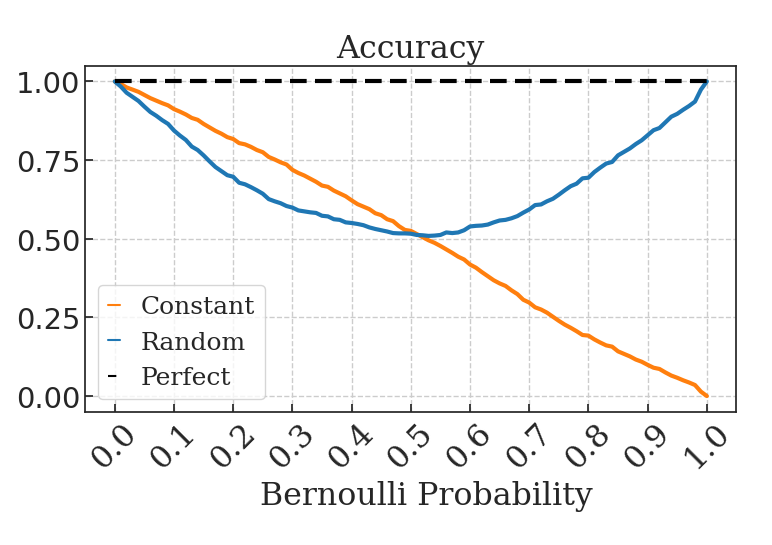
\includegraphics[width=\textwidth]{img/results_discussion/empirical/artificial_acc_final.png}
    \end{subfigure}
    \hfill
    \begin{subfigure}[b]{0.45\textwidth}
        \centering
        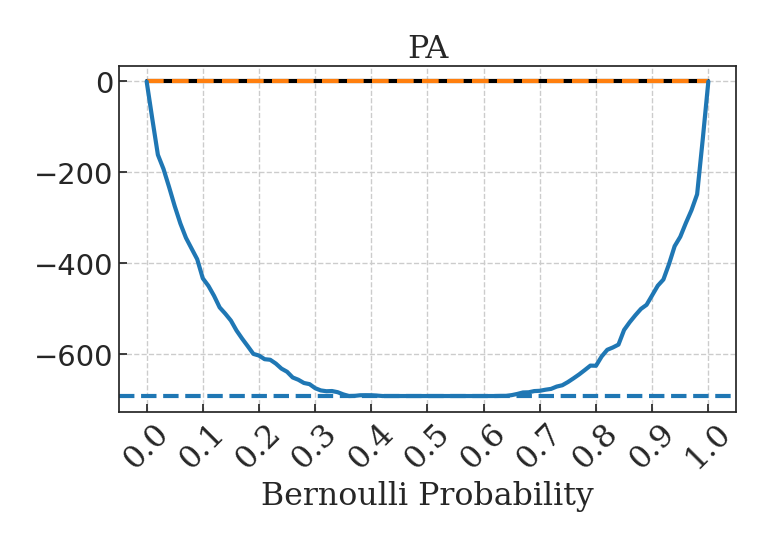
\includegraphics[width=\textwidth]{img/results_discussion/empirical/artificial_logPA_final.png}
    \end{subfigure}
    \caption{
    Evolution of PA and accuracy for constant, perfect and random classifiers across different 
    values of $p \in [0,1]$. Accuracy does not comply with the desired properties of a robustness metric
    and provides an inconsistent assessment that is exclusively driven by task performance. In contrast,
    PA continuously discriminates robust from unrobust classifiers for $p \in (0,1)$ and reaches 
    its minimum (blue dashed line) for the random classifier when $p \in (0.3,0.7)$.
    }
    \label{fig:empirical_plot}
\end{figure}

Table \ref{tab:empirical_table} displays the values of PA and accuracy
obtained for the case $p = 1/2$. It is clear that PA is independent of the task performance
of the model, which in classification tasks is mostly reported through accuracy-based metrics, and 
instead discriminates effectively the random classifier from the rest. In particular, 
PA converges towards its minimum value $-N \log{2}$ for the random classifier 
as $\beta \longrightarrow 0$, and converges towards zero for the 
other two as $\beta \longrightarrow \infty$. This behavior aligns with the 
intuitive assessment given in Example \ref{example:robustness}, since perfect and constant 
classifiers are robust by definition, while random classifiers are extremely unrobust. \\

 It can be observed that the miniumum PA is obtained only after 
a certain mismatch threshold has been reached, of approximately 30\% of the samples. 
This illustrates the trade-off navigated during $\beta$ optimization, in which 
matching samples are more heavily penalized the higher the value of $\beta$ is,
whereas mismatching samples are more heavily penalized the lower the value of $\beta$ is.
A balanced random classifier (i.e. balanced on the two classes) would yield the minimum
PA value for any possible original sample, as shown in the blue dashed line.\\

Figure \ref{fig:empirical_plot} extends these results across different values of 
$p \in [0,1]$. It can be observed that the minimum PA is obtained only after a mismatch 
threshold of approximately 30\% of the samples has been reached. This illustrates the 
trade-off navigated during $\beta$ optimization, where matching samples are increasingly penalized 
as the value of $\beta$ increases, while mismatching samples are more heavily penalized 
as $\beta$ decreases. FINISH. \\

The prediction confidence, expressed as a difference in  the unnormalized log-odds $\bm{F}$, 
is very informative with regard to the quality of the model, as we can intuitively infer that the latent 
space represented by a high-confidence model encodes a better set of features 
to discriminate observation classes than one with a lower prediction confidence. \\

HERE INTERPRETATION OF INFORMATIVENESS AND BETA. ALSO HERE INTERPRETATION OF BETA CONVERGENCE AND 
WHY WE DONT SET THE VALUE TO ZERO. HERE INTERPRETATION OF INFORMATIVENESS AND BETA. 
ALSO HERE INTERPRETATION OF BETA CONVERGENCE AND WHY WE DONT SET THE VALUE TO ZERO.
These and other results (see Appendix \ref{subsec:appendix_empirical_behaviour}) indicate
that the PA kernel behaves as expected and is highly informative of the generalization
capabilities of the model, provided that the nature of the randomness existing
between $\bm{x}^\prime$ and $\bm{x}^{\prime \prime}$ is known. \\

\begin{figure}[t]
    \centering
    \begin{subfigure}[b]{0.45\textwidth}
        \centering
        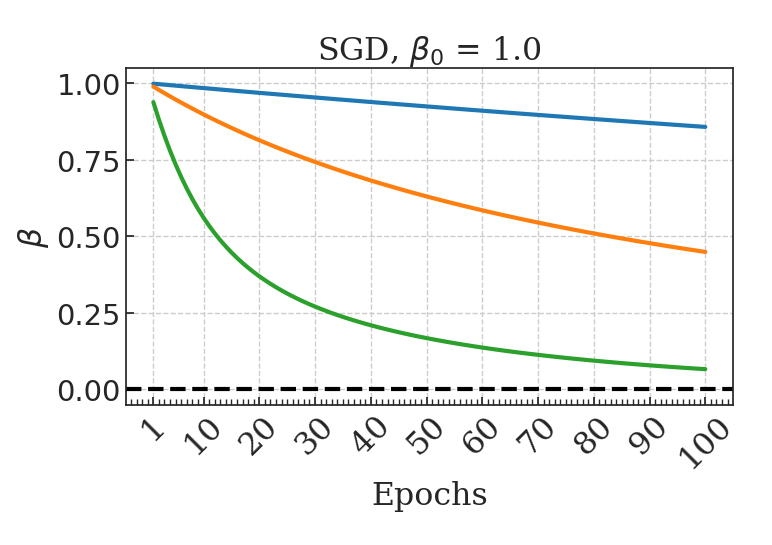
\includegraphics[width=\textwidth]{img/results_discussion/empirical/nonrob_met=betas_hue=ldiff.png}
    \end{subfigure}
    \hfill
    \begin{subfigure}[b]{0.45\textwidth}
        \centering
        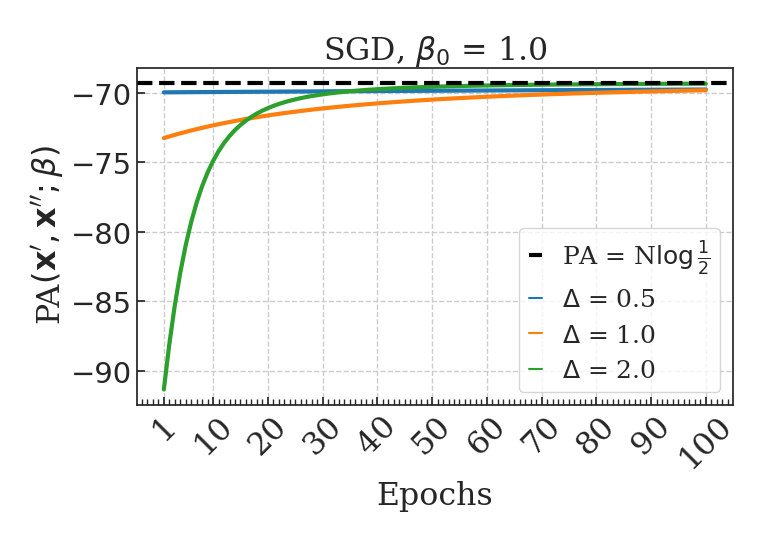
\includegraphics[width=\textwidth]{img/results_discussion/empirical/nonrob_met=logPA_hue=ldiff.png}
    \end{subfigure}
    \caption{Evolution of PA kernel optimization under different levels of prediction 
    confidence. An illustration of the original log-odds and its associated posterior distribution
    can be found in Appendix \ref{subsec:appendix_empirical_behaviour}.}
    \label{fig:prediction_confidence}
\end{figure}

The results obtained with artificial samples motivate the exploration of more realistic
scenarios. In general, the PA metric is expected to capture the generalization capabilities
of any model yielding probabilistic predictions, regardless of the task at hand. This
already represents an incredible advantage from an epistemological perspective, as we
can argue that the metric is agnostic of the underlying mechanism that generated the data
and even to the nature of the data itself. \\

In order to verify this claim, we will start by evaluating the robustness of two
different classifier models in two different domains under increasing levels of 
random noise. This particular setting, even if synthetically designed, is 
relevant in any classification context because it provides a general measure of the 
quality of the features learned. The presence of noise, at least 
at low levels, does not perturb the set of features that define a particular class from
a perceptual standpoint and should therefore not perturb very significantly the
predictions of robust models.

\begin{experiment}
The model under consideration is an image classifier for CIFAR10, a popular
computer vision dataset composed of coloured, 32 $\times$ 32 pixel images belonging to 10
different classes \cite{krizhevskyLearningMultipleLayers}. Sample
$\bm{x}'$ contains 10.000 images and $\bm{x}''$ is generated 
by perturbing each image with white noise of increasing intensity.
A pre-trained, undefended WideResNet-28-10
\cite{BMVC2016_87}
architecture is used to evaluate the effectiveness of the attack. The 
magnitude of the perturbations is expressed in the same terms as those 
of an adversarial attack for further reference, but translate to 
using $\sigma = 3 \ell_\infty$, as 99.73\% of the
total mass of the gaussian distribution lies within the 
interval $\pm 3\sigma$.
\end{experiment}

\begin{figure}[b]
    \centering
    \begin{subfigure}[b]{0.45\textwidth}
        \centering
        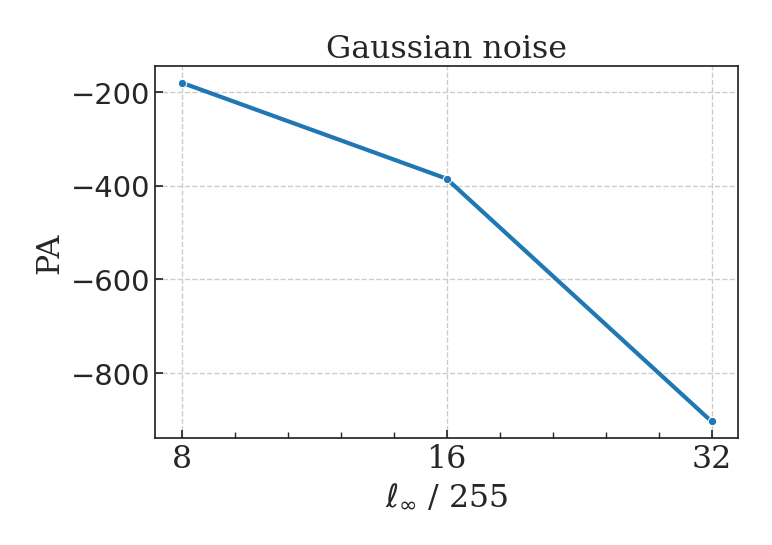
\includegraphics[width=\textwidth]{img/results_discussion/adversarial/GAUSSIAN_logPA_eps_single.png}
    \end{subfigure}
    \hfill
    \begin{subfigure}[b]{0.45\textwidth}
        \centering
        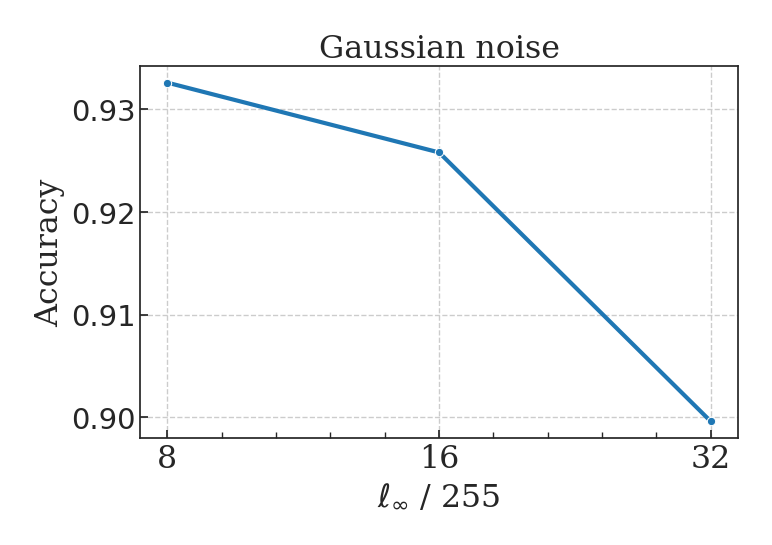
\includegraphics[width=\textwidth]{img/results_discussion/adversarial/GAUSSIAN_acc_pa_eps_single.png}
    \end{subfigure}
    \caption{PA and accuracy displayed by the CIFAR10 classifier under increasing levels of white noise. Robustness
    and task performance are shown to be non-linearly related.
    }
    \label{fig:gaussian_noise}
\end{figure}



Figure \ref{fig:gaussian_noise} shows that 
PA is highly sensitive to the presence of white noise and effectively captures the factor 
of increase in the magnitude of the perturbations. In general, gaussian perturbations genuinely simulate increasing levels of sampling randomness, as the 
perceptual features that should drive the inductive bias of the model are still present, even 
if in a proportionally dissimilar way as they were encoded. In contrast to adversarial attacks, 
these perturbations are not expected to distort the predictive outcome 
abruptly. As a result, any robustness score will be driven by the standard generalization error, including validation 
accuracy. \\

Figure \ref{fig:gaussian_optimization} expands these results by gradually adjusting
the perturbation so that it only affects a specific ratio of observations. As expected, 
$\beta \longrightarrow \infty$ in the unperturbed case, and converges
quickly to its optimal value in the rest of cases, even for a considerably large 
sample size. The decay in the PA value is less pronounced the higher
fraction of perturbed samples are there, which is consistent with the concept 
of robustness defined, as it already approaches the lower bound for these kinds of 
perturbation even when the whole sample has yet not been affected. \\


\begin{figure}[t]
    \centering
    \begin{subfigure}[b]{0.49\textwidth}
        \centering
        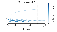
\includegraphics[width=\textwidth]{img/results_discussion/empirical/beta_100.pdf}
    \end{subfigure}
    \hfill
    \begin{subfigure}[b]{0.49\textwidth}
        \centering
        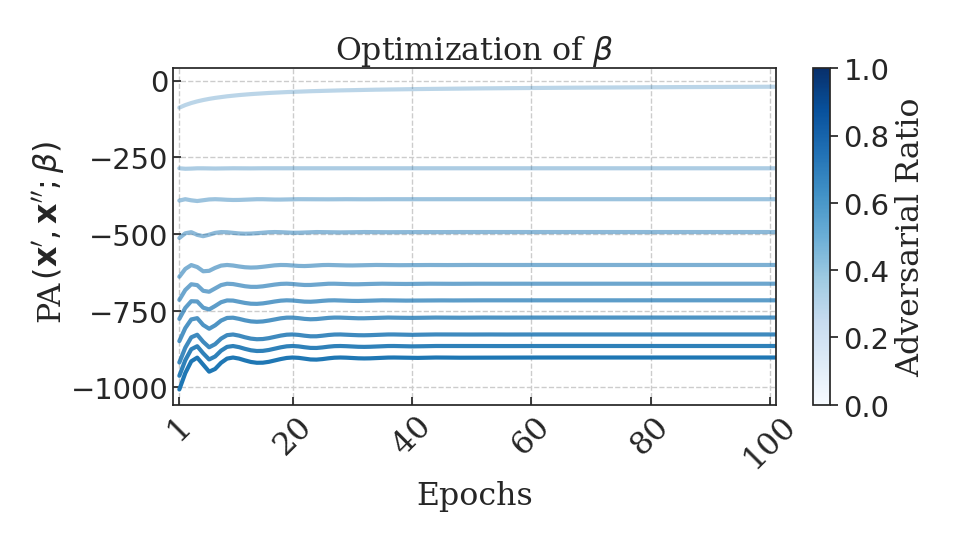
\includegraphics[width=\textwidth]{img/results_discussion/empirical/logPA_100.png}
    \end{subfigure}
    \caption{PA kernel optimization in the CIFAR10 gaussian noise setting for different ratio
    of perturbed samples. Perturbation magnitude is $\ell_\infty$ = 32 / 255.}
    \label{fig:gaussian_optimization}
\end{figure}



\begin{experiment}
The model under consideration is a sentiment classifier for IMDB,
a popular NLP dataset containing 50,000 movie reviews labeled 
as either positive or negative
\cite{maas2011learning}. 
A pre-trained DistilBERT-based architecture 
is adopted, with the appropiate tokenizer
\cite{sanh2019distilbert}. 
After a 100 epoch training using SGD with a learning rate of $10^{-3}$, the model with the highest validation
accuracy is selected. Then, the original test dataset $\bm{x}^\prime$
is incrementally perturbed to generate $\bm{x}^{\prime \prime}$, by either adding, removing or replacing 
single characters. This perturbation amounts to increasing the Levenshtein
distance $L$ between identical observations of the dataset, and the attack power
is defined as $2^{L}$.
\end{experiment}

\begin{figure}[b]
    \centering
    \begin{subfigure}[b]{0.45\textwidth}
        \centering
        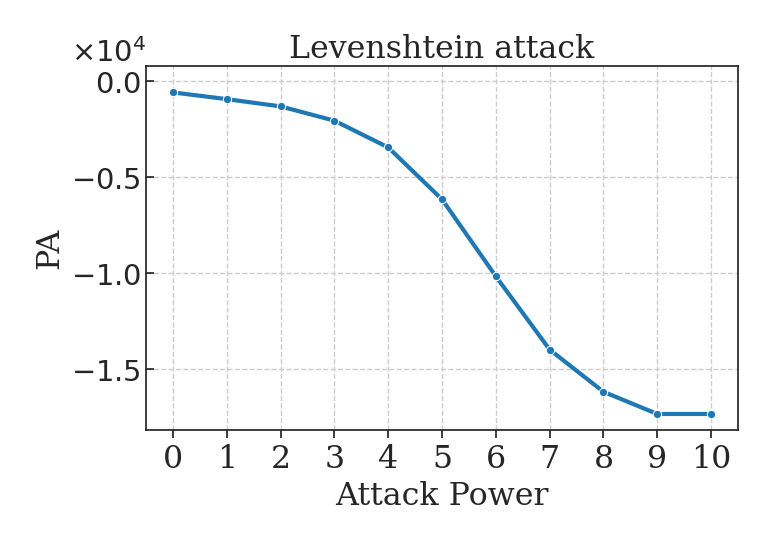
\includegraphics[width=\textwidth]{img/results_discussion/empirical/levenshtein_logPA.png}
    \end{subfigure}
    \hfill
    \begin{subfigure}[b]{0.45\textwidth}
        \centering
        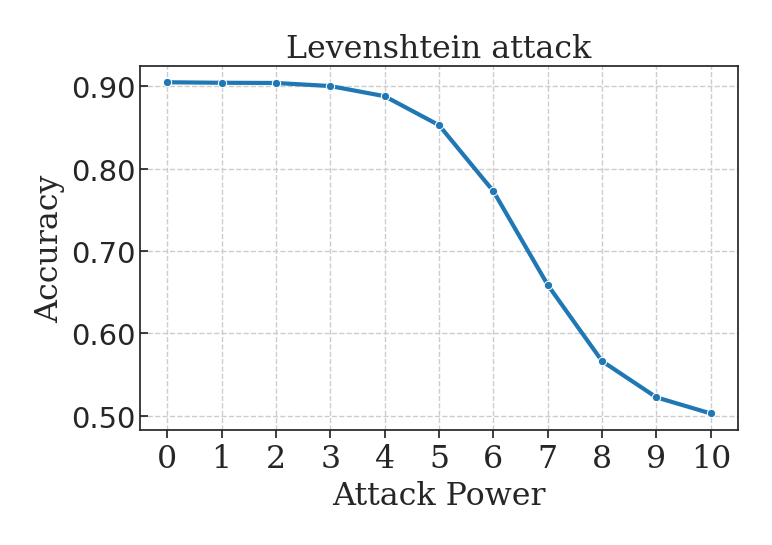
\includegraphics[width=\textwidth]{img/results_discussion/empirical/levenshtein_AFR_true.png}
    \end{subfigure}
    \caption{PA and accuracy for the IMDB sentiment classification under Levenshtein perturbations.
    The attack power is defined as $2^L$, being $L$ the Levenshtein distance between pairs of
    observations in $\bm{x}^\prime$ and $\bm{x}^{\prime\prime}$.}
    \label{fig:imdb_levenshtein}
\end{figure}

Figure \ref{fig:imdb_levenshtein} shows that PA is highly sensitive to the
presence of Levenshtein perturbations, as it is able to capture the
change in the predictive outcome of the model even when performance remains 
unaltered. In particular, accuracy remains maximum even when 4 characters
are perturbed in every observation, and begins to decrease only after that. In contrast,
PA drops significantly after the first perturbation and reaches its minimum value
after $2^9$ perturbations have been made, indicating that the outcome is maximally
unrobust. \\

Further discrepancies between accuracy and PA can be observed if the 
attack is designed to directly influence the sentiment prediction, which corresponds
to an adversarial setting. For instance, Figure \ref{fig:imdb_adversarial} shows that accuracy can be 
manipulated to increase or decrease by perturbing original samples with
adjectives that reinforce or contradict, respectively, 
the sentiment expressed in the review. In both cases, PA measures the lack of robustness in the
predictions that these perturbations represent, regardless of the task
performance displayed. The robustness against of adversarial attacks in
image classification tasks will be discussed in the next section. \\

\section{Adversarial setting}\label{sec:results_adversarial}

The first scenario in which covariate shift robustness will be measured is the
adversarial case. This setting serves as an archetypal use case for a robustness 
metric, given that adversarial perturbations are deliberately generated to mislead the
model, and any robustness score will ultimately be driven by the effectiveness of the 
attack. In particular, PA should be highly informative about the defensive capabilities 
of models, as the posterior distribution over the hypothesis class will shift 
significantly in the presence of adversarial perturbations. This section aims to validate 
this claim and provide deeper insights into the nature of the metric. \\

It is important to note that adversarial perturbations constitute an
intermediate instance between sampling randomness and distribution shift. 
On the one hand, they emulate a sampling variation that appears 
as an outlier under the model's representation of the true class, even if
the source of variability is completely artificial. On the other
hand, samples are known to contain the set of features that should 
align with the inductive bias of the model, and so the model's ability to 
distillate those features is in question. In practice, we are evaluating the 
quality of the complex discriminator function defining a basin of stability
around original samples, and for that no deep understanding of the nature of 
the randomness of the samples or the features they encode is needed.\\

This interpretation is aligned with the measure provided by accuracy-based metrics, 
because adversarial examples do not entail any accountable source of randomness, 
but instead exploit specific vulnerabilities of models to alter the position of the 
maximum of the posterior ditribution. A greater posterior overlap will still
indicate higher robustness to attacks, regardless of the nature of the model or the
attack, but optimal posteriors are expected to converge to very peaked gibbs
distributions centered at the predicted class, reducing the interpretability of PA
to that of accuracy. \\

In order to explore these claims, robustness and performance results will be
provided through the attack failure rate (AFR) value and compared to those
yielded by PA. The AFR computed with the true class labels will be used as a baseline
of model performance, whereas the AFR computed with the predicted class label
will be a reference for robustness, as it aligns with the aforementioned
interpretation.

\begin{definition}[\emph{Attack failure rate}]
    Let $\bm{\hat{y}^\prime}, \bm{\hat{y}^{\prime\prime}} \in \mathcal{Y}^N$ be the predicted class 
    labels for $\bm{x}^\prime$ and $\bm{x}^{\prime \prime}$, respectively, 
    and let $\bm{y}\in \mathcal{Y}^N$ be the true labels. Considering the definition of accuracy
    provided in Section \ref{sec:robustness_to_covariate_shift}, the attack failure rate (AFR)
    can be expressed as

    $$
    \begin{aligned}
        \operatorname{AFR}_\text{T} &= \operatorname{Accuracy}(\bm{\hat{y}^{\prime \prime}}, \bm{y}), \\
        \operatorname{AFR}_\text{P} &= \operatorname{Accuracy}(\bm{\hat{y}^{\prime \prime}}, \bm{\hat{y}^{\prime}}).
    \end{aligned}
    $$

\end{definition}

\begin{definition}[\emph{Adversarial ratio}]
    Besides the maximum norm allowed for each perturbation, we are also interested in evaluating 
    the sensitivity of our robustness measure to the ratio of perturbed samples in the dataset, 
    also known as adversarial ratio $\alpha \in [0,1]$. The final adversarial dataset $\bm{x}''$ will be generated as

    $$
    \bm{x}'' := \alpha \bm{x}'' + (1 - \alpha) \bm{x}',
    $$

    where $\bm{x}'' = \bm{x}' + \bm{\Delta}$, as per Definition \ref{def:adversarial_perturbation}.
\end{definition}

This incremental expansion of the attack is particularly relevant for PA, as we would initially 
expect it to behave non-linearly with respect to $\alpha$ and converge faster to
the the $\alpha=1$ robustness value than any accuracy-based metric, in light of the results obtained
in the previous section. \\

Before delving into the results, it is worth exploring the immediate consequences
of the previous claim, namely the fact that the maximum posterior agreement will
be achieved when gibbs distributions are highly peaked on the predicted 
class, at least for moderate attacks. This is because most adversarial 
perturbations will not succeed at misleading the model and thus drive the inverse temperature to
infinity. The divergence of $\beta^{*}$ is only limited by the set of misleading adversarial 
examples, that for being perturbed from the original class are still expected to assign a
significant confidence to the original prediction, even if not the maximum anymore.
Table \ref{tab:entropy_gibbs} illustrates this claim by showing that $\beta^{*} > 1$ 
for all robust models, resulting in a substantial decrease of the entropy between initial and 
optimal posteriors. \\

This realization allows us to break down the dataset into subsets of observations
that contribute to the final PA value in different ways, and therefore improve
the interpretation of the resulting robustness measurement.
For a start, a robust model should be expected to correctly classify most of the 
original observations with high confidence, as they
contain the features encoded in the inductive bias of the 
classifier. Original samples that do not contain these features will be misclassified,
and the lack of generalization to sampling randomness should be penalized for lowering
the confidence in the predicted class. Regarding adversarial examples, a clear
distinction between robust and non-robust models should be made based on the success 
rate of perturbations and the confidence attributed to misleading predictions. Adversarial 
perturbations on originally misclassified observations will not be of much interest,
as the effect on prediction confidence should not be as significant as in
the correctly classified ones. An interpretable expression for PA in the adversarial
setting can be obained by approximating the optimal posterior for each of these
subsets of observations. \\

\begin{theorem}[\emph{Approximated PA in the adversarial setting}]
    Let $\Xi_{\text{ERR}}$, $\Xi_{\text{MIS}}$ and $\Xi_{\text{ADV}}$ be the approximated robustness
    contributions of correctly classified original samples, misclassified original samples
    and misleading adversarial samples, respectively. Then, we can express

    $$
    \operatorname{PA} \approx \Xi_{\text{ERR}} + \Xi_{\text{MIS}} + \Xi_{\text{ADV}} = \Xi_{\text{SAM}} + \Xi_{\text{ADV}} 
    $$

    with
    $$
    \begin{aligned}
        &\Xi_{\text{ERR}} = N \operatorname{AFR}_T^0 \operatorname{AFR}_P \log \left( 1 - 2\delta_{\text{ERR}} \right), \\
        &\Xi_{\text{MIS}} = N (1- \operatorname{AFR}_T^0) \operatorname{AFR}_P \log \left( 1 - 2\delta_{\text{MIS}} \right), \\
        &\Xi_{\text{ADV}} = N \operatorname{AFR}_T^0 (1 - \operatorname{AFR}_P) \log \delta_{\text{ADV}},
    \end{aligned}
    $$

    where $\operatorname{AFR}_T^0 \equiv \operatorname{AFR}_T(\alpha=0)$ is the accuracy of the model in the original data.
    Variables $\delta_{\text{ERR}}$, $\delta_{\text{MIS}}$ and $\delta_{\text{ADV}}$ account for the 
    average probability assigned to
    classes other than the predicted class for the three aforementioned cases 
    (see illustration in Figure \ref{fig:appendix_adv_illustration}). $\Xi_{\text{SAM}}$ aggregates
    the first two terms and will be interpreted as the sampling randomness contribution.
    \label{thm:approximated_pa}
\end{theorem}
\begin{proof}
    See Apendix \ref{sec:appendix_results_adversarial}.
\end{proof}

Figures \ref{fig:appendix_adversarial_approx_pa_pgd} and \ref{fig:appendix_adversarial_approx_pa_fmn}
compare the true and approximated PA values under increasing adversarial ratio for
PGD and FMN attacks, respectively. It is clear that penalizations are overestimated, 
given that the average posterior probability was used and differences by defect are more 
significantly penalized than those by excess due to the nonlinear nature of the logarithm in 
the range $[0,1]$. Besides, $\beta^{*}$ is fixed to its lowest possible value (i.e. when $\alpha$ = 1),
which makes the approximation on the FMN attack less reliable for smaller adversarial 
ratio settings, as $\beta^{*}$ decreases significantly due to the effectiveness of the attack. \\

Nevertheless, the relative differences in the approximated PA values are consistent
with the true values, and the ranking of the models is largely preserved across different
$\alpha$ values. For that reason, the additional interpretability provided by this approximation
will illustrat PA expression will help characterize the source of the robust and unrobust
observed in the different models. \\

\begin{table}[t]
    \centering
        \begin{tabular}{l|rr|rr}
        Defense & $\beta^{*}_{\text{PGD}}$ & $\Delta H_{\text{PGD}}$  & $\beta^{*}_{\text{FMN}}$ & $\Delta H_{\text{FMN}}$ \\
        \midrule
        {\color{tab:orange} \textbf{Undefended}} & 0.78 & 0.048 & 0.65 & 0.10\\
        {\color{tab:blue} \textbf{Engstrom et al.}} & 15.63 & -1.204 & 2.59 & -0.71\\
        {\color{tab:green} \textbf{Athalye et al.}} & 35.48 & -3.049 & 19.84 & -2.13 \\
        {\color{tab:red} \textbf{Wong et al.}} & 15.46 & -1.229 & 4.59 & -0.96\\
        {\color{tab:purple} \textbf{Addepalli et al.}} & 15.89 & -2.023 & 6.08 & -1.71 \\
        {\color{tab:brown} \textbf{Wang et al.}} & 11.24 & -1.833 & 2.53 & -1.41\\
        \bottomrule
        \end{tabular}
        \caption{
        Entropy difference $\Delta H = H(\beta^{*}) - H(1)$
        for different models, obtained for FMN and $\ell_\infty$ = 8/255 
        PGD attacks, both at $\alpha = 1$. Entropy values are 
        estimated using the average posterior distribution over correctly classified
        samples, which constitute the largest proportion of the dataset.
        Figures \ref{fig:pgd_distributions_undefended}-\ref{fig:pgd_distributions_bpda}
        show the initial and optimal average posteriors from which these values
        were computed.
        }
        \label{tab:entropy_gibbs}
\end{table}

\begin{experiment}
The results provided in this section have been obtained using the CIFAR10 dataset
\cite{krizhevskyLearningMultipleLayers},
which is widely regarded as a standard benchmark for robustness evaluation. CIFAR10 is
a balanced dataset containing 60.000 coloured 32 $\times$ 32 pixel images belonging to 10
different classes. We will consider a pre-trained WideResNet-28-10
\cite{BMVC2016_87}
as a baseline, undefended model and compare it to some state-of-the-art robust ResNet50
\cite{resnet50}
models provided by the 
RobustBench \cite{croceRobustBenchStandardizedAdversarial2021a}
library under PGD \cite{madryDeepLearningModels2019}
and FMN \cite{pintorFastMinimumnormAdversarial2021}
attacks, both run for 1000 steps (see Section \ref{sec:adversarial_setting}).
The defenses applied are those proposed by 
{\color{tab:blue} \textbf{Engstrom et al.}} \cite{engstrom2019adversarial}, 
{\color{tab:green} \textbf{Athalye et al.}} \cite{AthalyeC018}, 
{\color{tab:red} \textbf{Wong et al.}} \cite{WongRK20}, 
{\color{tab:purple} \textbf{Addepalli et al.}} \cite{Addepalli2022ScalingAT}
and {\color{tab:brown} \textbf{Wang et al.}} \cite{wang2023betterdiffusionmodelsimprove}.
The PGD attack power will be specified in terms of $\ell_\infty$, which corresponds
to the maximum perturbation allowed for each pixel. This is consistent with the characterization
of adversarial perturbation given in the previous chapter, as every perturbation will be bounded
to the region defined by $\mathbf{B}_\infty^{\ell_{\infty}} (x)$.
\end{experiment}

\begin{figure}[H]
    \centering
    \begin{subfigure}[b]{0.25\textwidth}
        \centering
        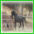
\includegraphics[width=\textwidth]{img/results_discussion/adversarial/adv_unperturbed_framed.png}
        \caption{Original}
    \end{subfigure}
    \hfill
    \begin{subfigure}[b]{0.25\textwidth}
        \centering
        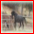
\includegraphics[width=\textwidth]{img/results_discussion/adversarial/adv_pgd_framed.png}
        \caption{PGD, $\ell_\infty$ = 36/255}
    \end{subfigure}
    \hfill
    \begin{subfigure}[b]{0.25\textwidth}
        \centering
        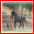
\includegraphics[width=\textwidth]{img/results_discussion/adversarial/adv_fmn_framed.png}
        \caption{FMN}
    \end{subfigure}
    \caption{Original and adversarially-perturbed CIFAR10 sample of class \texttt{horse}. Both perturbations succeed
    at misleading an undefended, pre-trained WideResNet-28-10 architecture.}
\end{figure}

The first results presented correspond to PGD attacks with different attack power 
$\ell_\infty$, namely 8/255, 16/255 and 32/255, for increasing ratio of 
perturbed samples in the CIFAR10 dataset.

\begin{figure}[H]
    \centering
    \begin{subfigure}[b]{\textwidth}
        \centering
        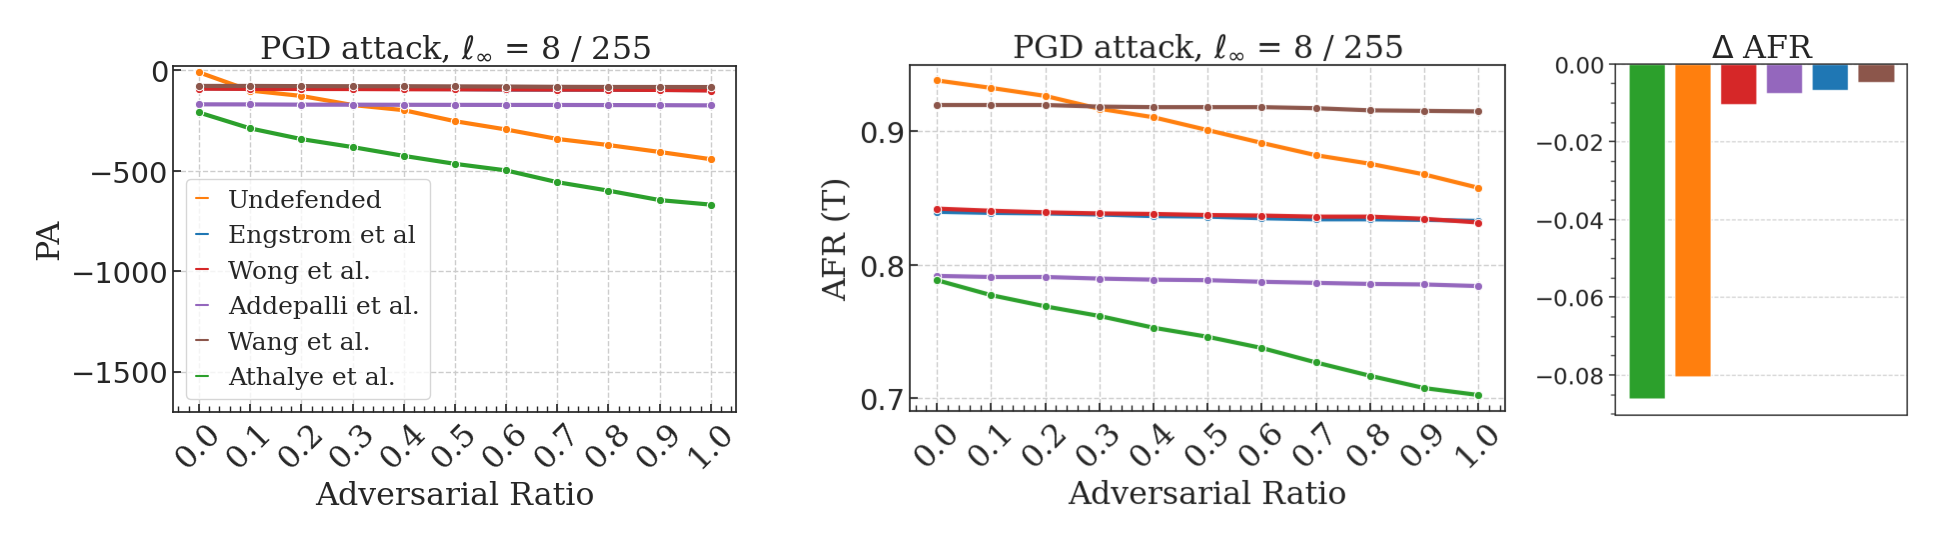
\includegraphics[width=\textwidth]{img/results_discussion/adversarial/PGD_0.0314_combo.png}
    \end{subfigure}

    \vspace{1em}

    \begin{subfigure}[b]{\textwidth}
        \centering
        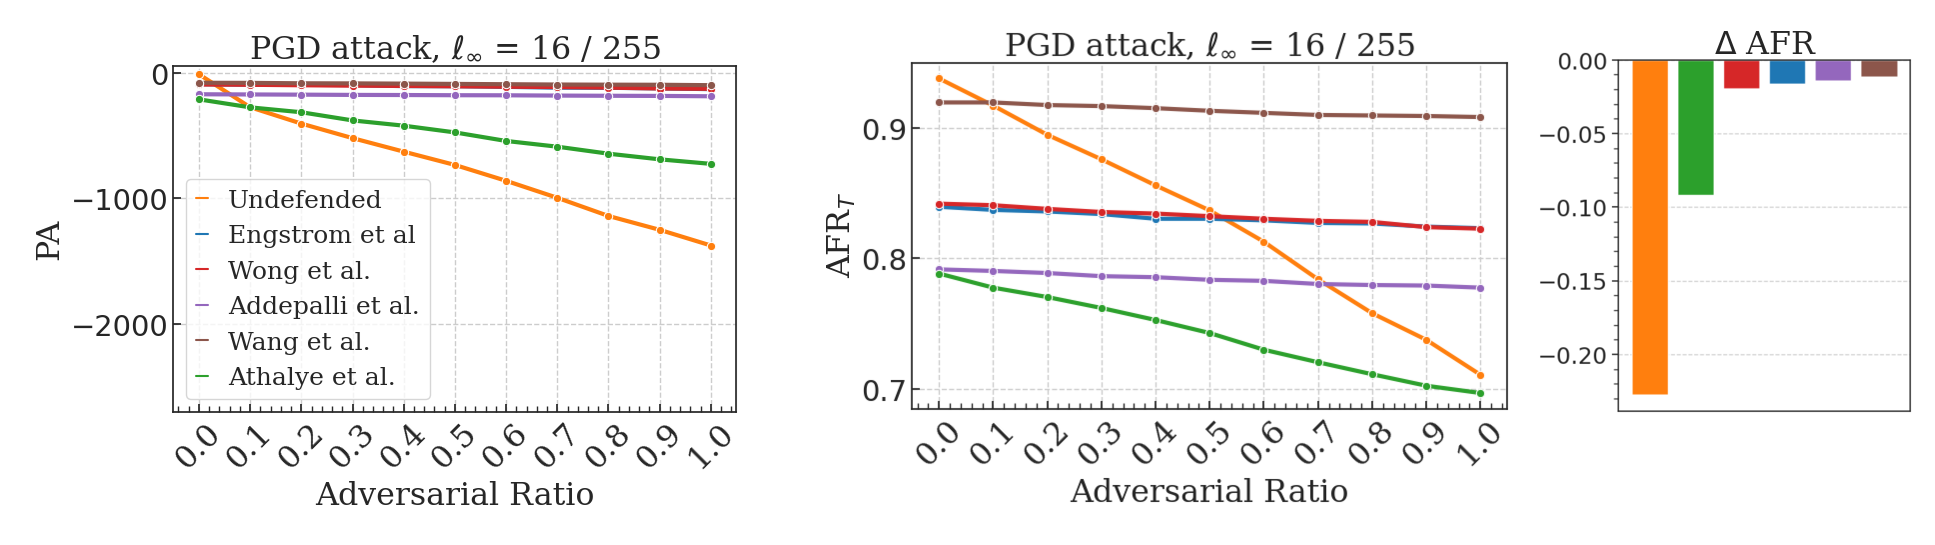
\includegraphics[width=\textwidth]{img/results_discussion/adversarial/PGD_0.0627_combo.png}
    \end{subfigure}

    \vspace{1em}

    \begin{subfigure}[b]{\textwidth}
        \centering
        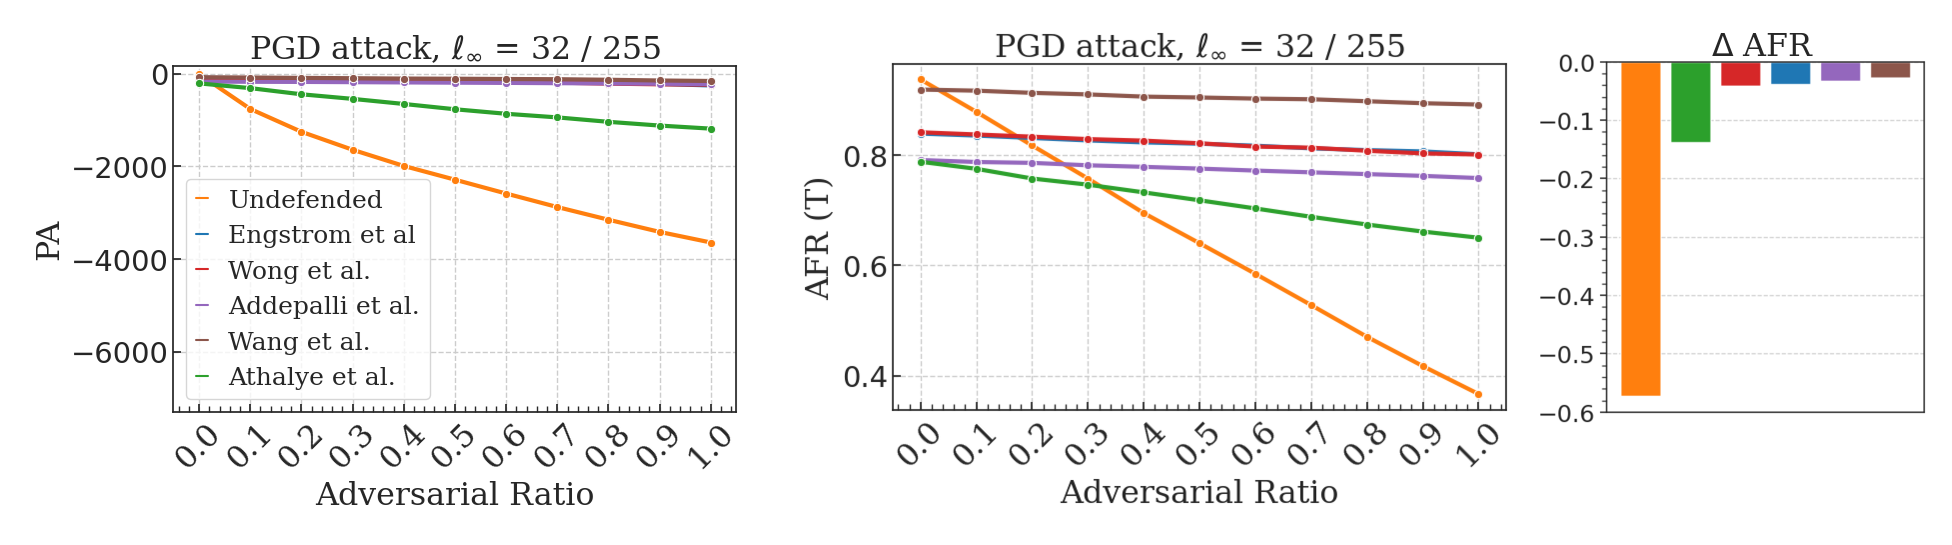
\includegraphics[width=\textwidth]{img/results_discussion/adversarial/PGD_0.1255_combo.png}
    \end{subfigure}

    \caption{PA, $\operatorname{AFR}_\text{T}$ and the AFR variation against increasing adversarial ratio $\alpha \in [0,1]$ at different
    perturbation norm bounds $\ell_infty$. A pre-trained, undefended WideResNet-28-10
    and five RobustBench %\cite{croceRobustBenchStandardizedAdversarial2021a}
    defended models are subject to a 1000 step PGD attack.
    When $\alpha$ = 0, $\operatorname{PA} \longrightarrow 0$ as $\beta \longrightarrow \infty$ in all cases, but
    the convergence rate depends on the prediction confidence (see Figure \ref{fig:prediction_confidence}) and thus yields an assessment equivalent to that
    of $\operatorname{AFR}_\text{T}$.
    }
    \label{fig:six_figures_pa_adv}
\end{figure}

At first glance, it is clear that PA is able to discriminate robust models from
the {\color{tab:orange} \textbf{Undefended}} one, which is shown to significantly
decrease its performance with increasing adversarial ratio and attack power. As expected, 
the rate at which its performance decreases is higher
the more powerful the attack is, since a greater percentage of samples are able to
mislead its predictions. \\

From both PA and $\operatorname{AFR}_{\text{T}}$ stems the fact that {\color{tab:green} \textbf{Athalye et al.}}
is significantly less robust to PGD attacks than its RobustBench counterparts, as 
its performance decreases way more significantly with increasing adversarial ratio. 
We observe that the rate at which its performance decreases is inversely proportional to the 
attack power. This is consistent with the behaviour expected from a JPEG compression defense 
mechanism, as it is less effective for small perturbations \cite{dasKeepingBadGuys2017}. \\

A fundamental difference between these two models, which cannot be
inferred from a purely performance-based metric, is the nature of the misalignment in
the probabilistic output of the model, which is the source of the robust and non-robust
behaviour observed. Figure \ref{fig:unrobust_posterior_short_pgd} \textbf{(right)}
shows the optimal $\beta^{*}$ value for each model, which follows
the entropy of the posterior distribution and discriminates the two non-robust
models from the rest and from each other. The {\color{tab:orange} \textbf{Undefended}}
model provides overconfident predictions that maximize disagreement in misleading and 
misclassified samples, whereas {\color{tab:green} \textbf{Athalye et al.}} provides 
uncertain predictions that minimize disagreement in adversarial samples but have 
the opposite effect in correctly classified ones. \\

Following the interpretation outlined in Chapter \ref{sec:theory}, we show that $\beta^{*}$ effectively measures the quality of 
the informativeness estimation made by each model. The {\color{tab:orange} \textbf{Undefended}} 
model overestimates the information content of the features it has learned, and thus overfits 
to these and is unable to generalize under adversarial perturbations. On the other hand, 
{\color{tab:green} \textbf{Athalye et al.}} underestimates the information content and thus
provides overly uncertain predictions. The maximum mutual information between posteriors is 
lower than its robust counterparts for both models, the former because information is not 
mutual and the latter because there is less information.
This insight clarifies the unintuitive behaviour observed earlier, by which {\color{tab:green} \textbf{Athalye et al.}} 
robustness value decreases at a lower rate with increasing attack power, despite maintaining a
constant decrease in performance. \\

Figure \ref{fig:unrobust_posterior_short_pgd} \textbf{(left)} illustrates
the previous reasoning by displaying the average posterior
probability assigned to the predicted class by each model, conditioned on the type
of prediction assigned. This discrimination yields three groups of observations,
namely original samples that are correctly classified by the robust model, 
original samples that are misclassified, and perturbed samples that, having their 
associated unperturbed sample been correctly classified, 
have been able to mislead the model. These three cases are relevant from the 
adversarial robustness perspective,  as they illustrate the trade-off between high-confident 
original predictions and adversarial vulnerability, which has been already stated in 
previous chapters. {\color{tab:brown} \textbf{Wang et al.}}
acts as a reference for an ideal robust behaviour, in which original samples are
predicted with high confidence and adversarially misleading predicted labels are 
only slightly more likely than the rest. Equivalent representations for the remaining
models can be found in Figure \ref{fig:appendix_adversarial_distribution_pgd}.\\

\begin{figure}[H]
    \centering
    \begin{subfigure}[b]{\textwidth}
        \centering
        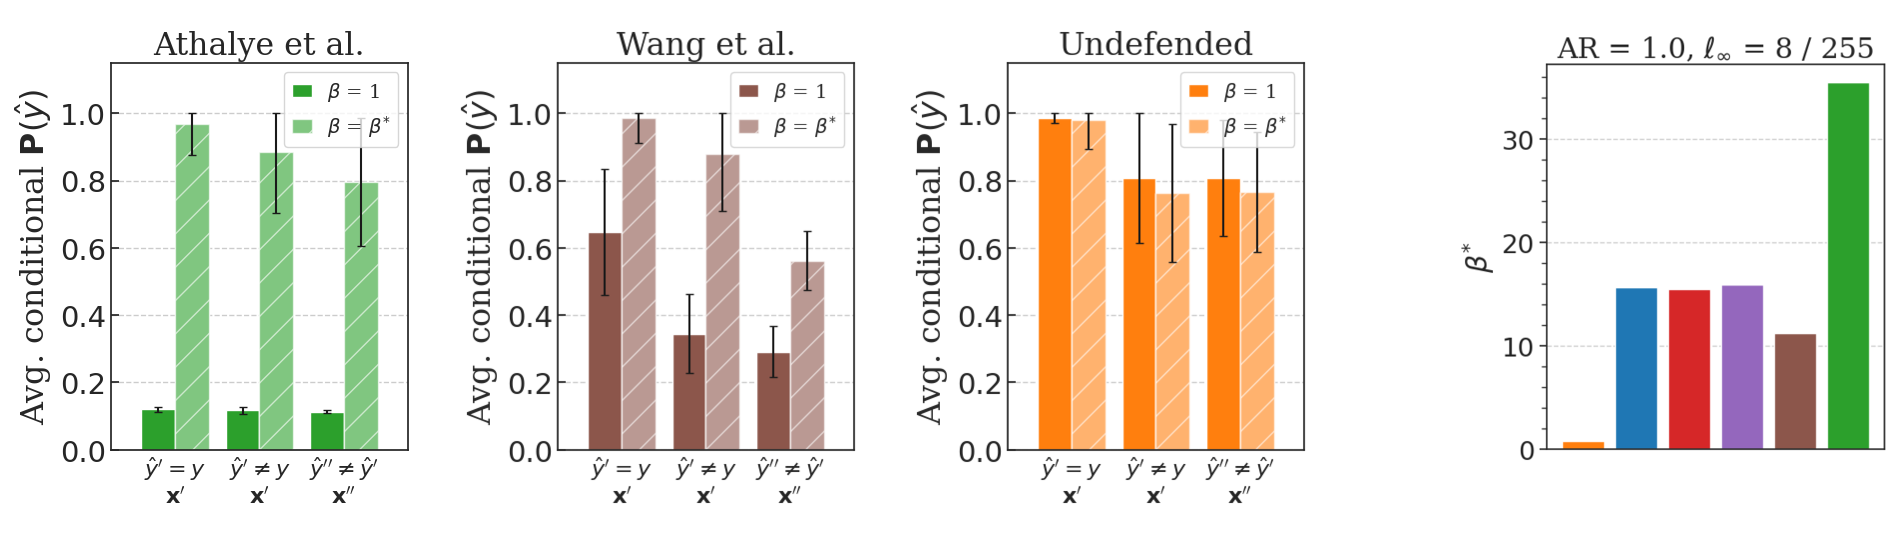
\includegraphics[width=\textwidth]{img/results_discussion/adversarial/bpda_wang_undefended_beta_pgd.png}
    \end{subfigure}
   
    \caption{(\textbf{left}) Average posterior probability of the predicted class for 
    correctly classified original samples, misclassified original samples, and 
    misleading adversarial samples, respectively. (\textbf{right}) Optimal $\beta^{*}$ value for each model.
    Results obtained through a PGD attack with $\ell_\infty = 8 / 255$.}
    \label{fig:unrobust_posterior_short_pgd}
\end{figure}

With respect to robust models, we observe a significant difference in the 
discriminative power of PA and accuracy-based metrics that does not immediately
derive from the informativeness of the optimal posterior. As remarked before, AFR (P)
constitutes our baseline robustness metric, as by definition represents the ratio
of predictions that remained constant under adversarial perturbations, and
therefore ranks models by their predictive capabilities against these attacks. The
value of $\Delta$AFR aligns with that definition, and discriminates robust models
by a very thin margin, selecting {\color{tab:brown} \textbf{Wang et al.}} as
the best. Further analysis on PA is needed to understand the source of this 
discrepancy, as for instance why {\color{tab:purple} \textbf{Addepalli et al.}} model
is attributed a significantly lower value than the remaining robust models
under a $\ell_\infty$ = 8/255 PGD attack, despite displaying a similar decrease in performance. \\

\begin{figure}[H]
    \centering
    \begin{subfigure}[b]{0.37\textwidth}
        \centering
        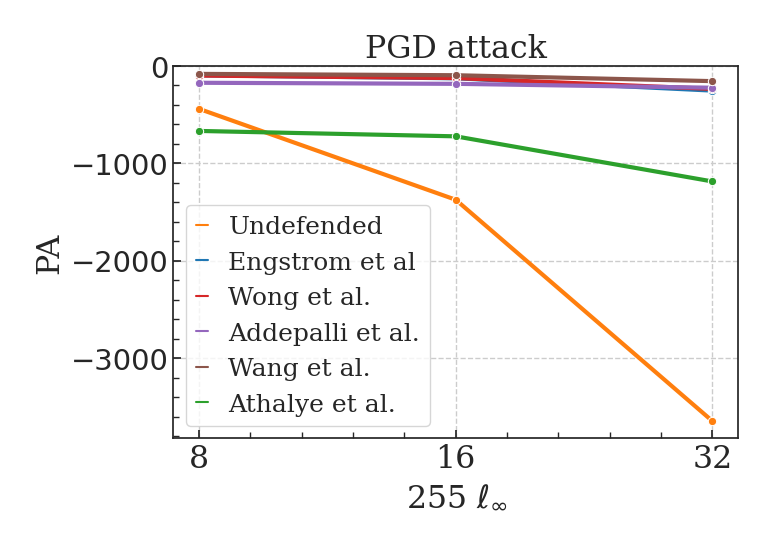
\includegraphics[width=\textwidth]{img/results_discussion/adversarial/PGD_logPA_eps.png}
    \end{subfigure}
    \hfill
    \begin{subfigure}[b]{0.59\textwidth}
        \centering
        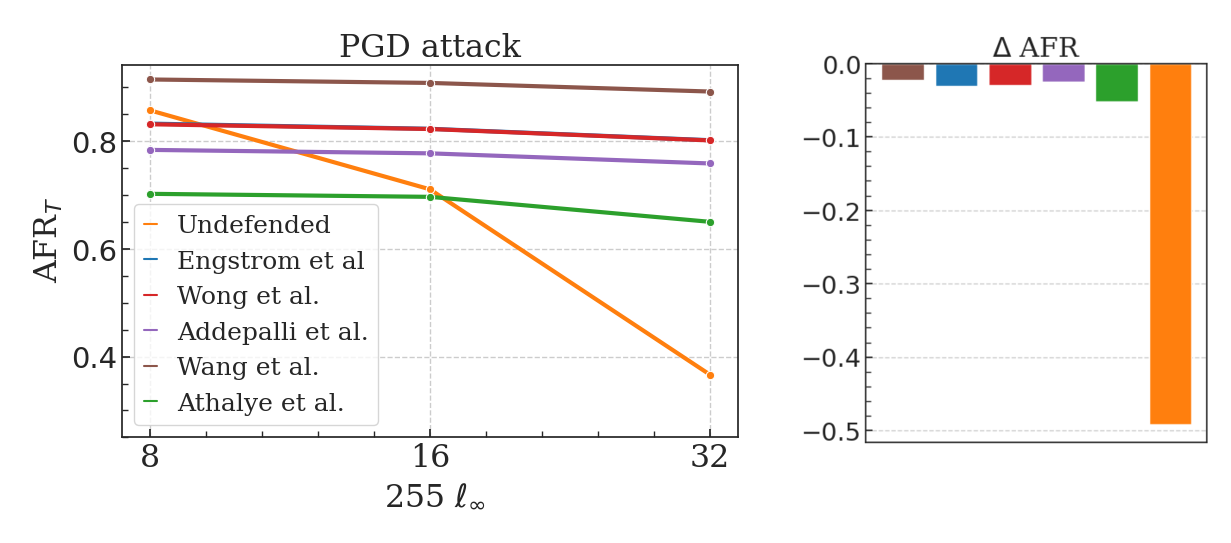
\includegraphics[width=\textwidth]{img/results_discussion/adversarial/PGD_AFR_true_eps_diff.png}
    \end{subfigure}
    \caption{PA, $\operatorname{AFR}_\text{T}$ and the AFR variation against increasing attack power for  $\alpha = 1$. 
    The aforementioned undefended net and several RobustBench robust models are considered
    under a 1000 step PGD attack.}
    \label{fig:pgd_eps}
\end{figure}

Finally, Figure \ref{fig:pgd_eps} shows that PA is also discriminative with respect to
increasing attack power, expressed through the maximum allowed $\ell_\infty$ norm. 
As mentioned earlier, PA values are heavily aligned with the performance
decrease of the models under a specific attack power, but the observed decrease in PA 
under increasing $\ell_\infty$ is much more significant that the decrease 
in performance. This can be explained by the fact that the metric is sensitive 
to the overall posterior shift and not only the position of the maximum. When increasing 
the attack power, confidence in the predicted class will decrease in general, 
even when the sample does not succeed at misleading the model, and therefore the
overall overlap between posteriors will be reduced even at comparable performance 
levels. This observation further illustrates the independent discriminability power
offered by PA (see Properties \ref{properties:robustness}), which constitutes the 
cornerstone argument of this work. \\

In order to widen the scope of the analysis, analogous results will be obtained for
FMN attacks, which are expected to be more effective than PGD attacks for being 
unbounded, which translates into an overall decrease in $\beta^{*}$ (see 
Table \ref{tab:entropy_gibbs}). Figure \ref{fig:adv_fmn_pa_afr} shows the evolution 
of PA against increasing adversarial ratio for the same models, and compares
it with the assessment provided by AFR.


\begin{figure}[H]
    \centering
    \begin{subfigure}[b]{0.39\textwidth}
        \centering
        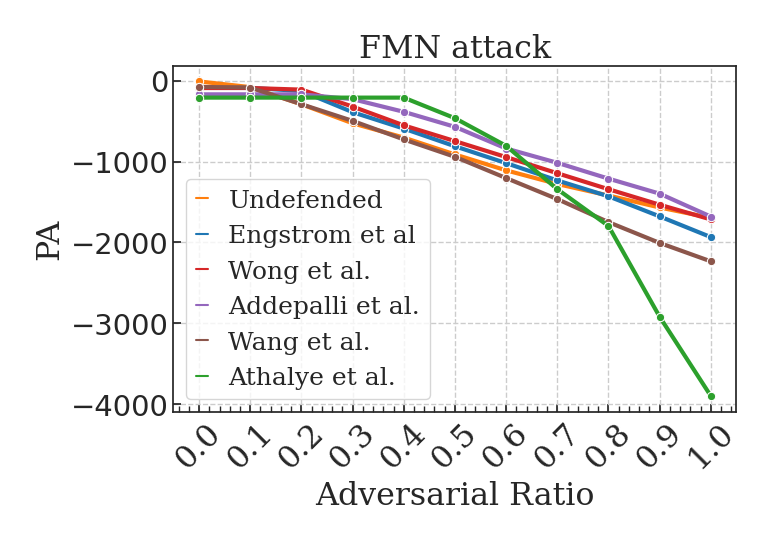
\includegraphics[width=\textwidth]{img/results_discussion/adversarial/FMN_logPA.png}
    \end{subfigure}
    \hfill
    \begin{subfigure}[b]{0.59\textwidth}
        \centering
        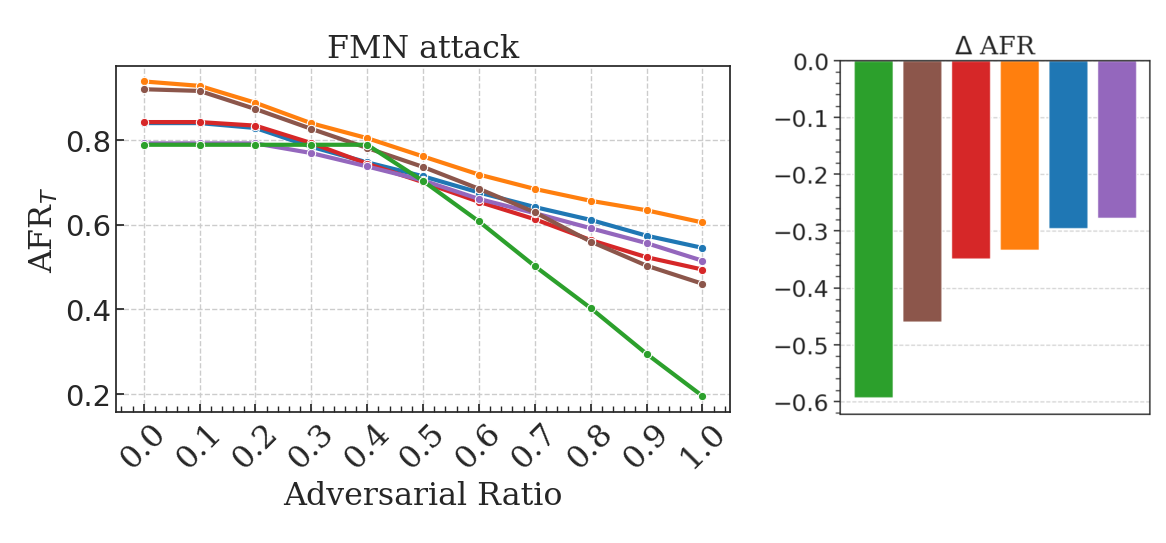
\includegraphics[width=\textwidth]{img/results_discussion/adversarial/FMN_1000_AFR_true.png}
    \end{subfigure}
    \caption{PA, $\operatorname{AFR}_\text{T}$ and the AFR variation against increasing adversarial ratio. 
    The aforementioned undefended net and several RobustBench robust models are considered 
    under a 1000 step FMN attack.}
    \label{fig:adv_fmn_pa_afr}
\end{figure}


As expected, the effectiveness of the FMN attack is superior to that of PGD attacks, as
the decrease in performance is substantially more significant for all models, especially the ones
previously considered robust. In this case, the assessment provided by PA is 

It is likely that these models have been defended with a
compression strategy that succeeds at filtering out small perturbations, which are
the ones employed by FMN, and for that reason maintain their performance at low
adversarial ratio values \cite{dasKeepingBadGuys2017}.
In particular, {\color{tab:green} \textbf{Athalye et al.}} remains maximally robust
until at least 40\% of the samples are perturbed, at which point the defensive strategy
is neutralized and a constant fraction of the additional perturbed samples succeeds at
misleading the model, which translates into a linear decrease in performance and PA. \\

PA proves to be very discriminative among robust models and to represent the 
phase transition entailed by the collapse of the defense strategy better than AFR does, which can be
observed in more detail in Figure \ref{fig:appendix_adversarial_afrpred_fmn}. A significative
result is that PA is not so directly aligned with $\Delta$AFR, in contrast to
the PGD case, which shows again that the decrease in performance is not the main driver of
the robustness assessment provided by PA, but instead can be interpreted as a consequence of
a misalignment in the posterior distributions of adversarial samples, which are the ones driving
the metric after the $\alpha$ thresold is reached. \\

\begin{figure}[H]
    \centering
    \begin{subfigure}[b]{\textwidth}
        \centering
        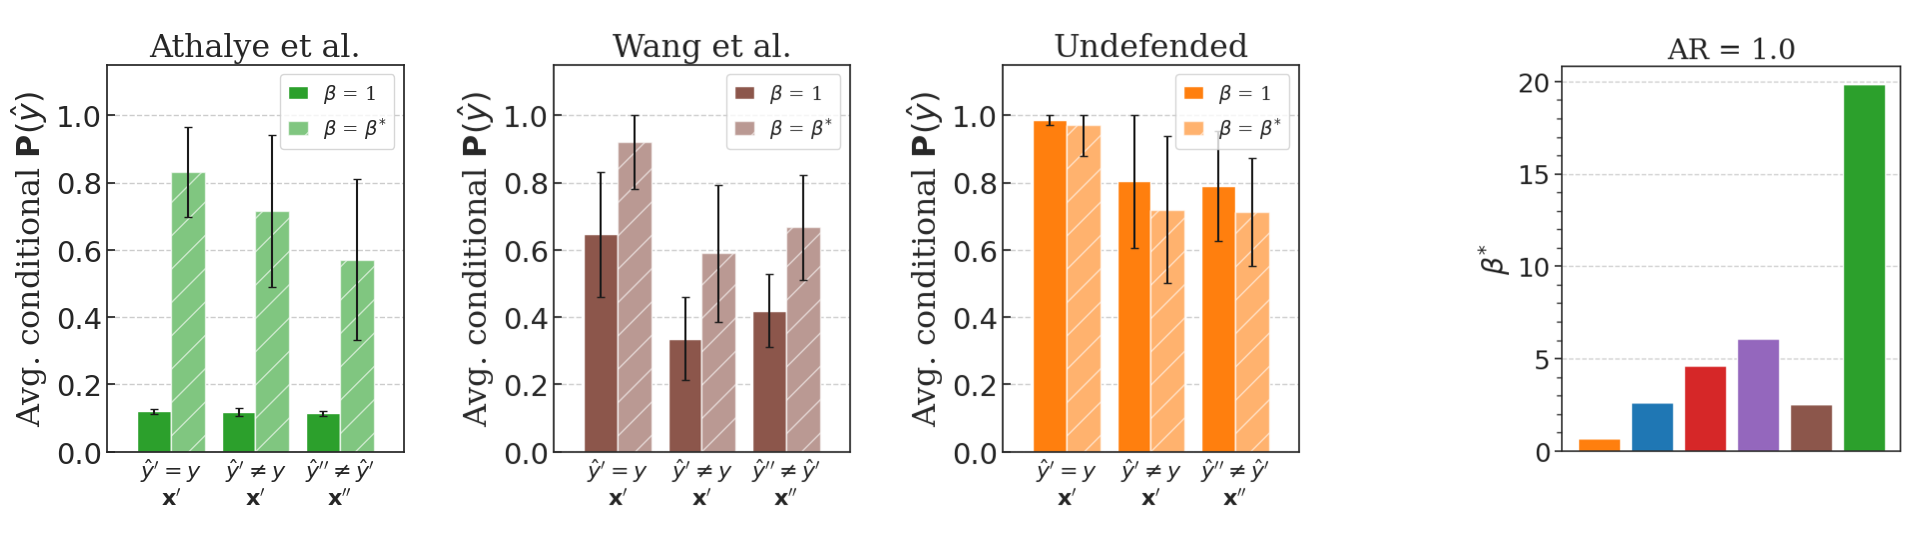
\includegraphics[width=\textwidth]{img/results_discussion/adversarial/bpda_wang_undefended_beta_fmn.png}
    \end{subfigure}
   
    \caption{(\textbf{left}) Average posterior probability of the predicted class for 
    correctly classified original samples, misclassified original samples, and 
    misleading adversarial samples, respectively. (\textbf{right}) Optimal $\beta^{*}$ value for each model.
    Results obtained through a FMN attack.}
    \label{fig:unrobust_posterior_short_fmn}
\end{figure}

Figure \ref{fig:unrobust_posterior_short_fmn} gives insight into the probabilistic output
of the model and the informativeness of the optimal posterior for the {\color{tab:orange} \textbf{Undefended}}, 
{\color{tab:green} \textbf{Athalye et al.}} and {\color{tab:brown} \textbf{Wang et al.}} models, in
analogous way to the PGD experiments. The first two models display a very similar behaviour for 
$\beta = 1$, but optimal posteriors are less informative due to the increased number of misleading
samples, which translates into a smaller $\beta^{*}$. The response of 
the {\color{tab:brown} \textbf{Wang et al.}} model further illustrates the higher effectiveness of
FMN attacks, as adversarial perturbations are on average more misleading than outlier samples in
the original dataset, which did not occur in the PGD case. Analogous representations for the remaining
models can be found in Figure \ref{fig:appendix_adversarial_distribution_fmn}, which show
that the {\color{tab:purple} \textbf{Addepalli et al.}} is the only robust model that maintains
the same behaviour under both attacks.\\

Overall, we recognize that PA has a higher discriminative power than AFR, especially
considering the evolution of each metric over increasing adversarial ratio, as
seen in Figures \ref{fig:six_figures_pa_adv} and \ref{fig:adv_fmn_pa_afr}. 
In particular, Figures \ref{fig:appendix_adversarial_afrpred_pgd} and \ref{fig:appendix_adversarial_afrpred_fmn}
compare the evolution of PA with that of AFR (P), which is the baseline metric for robustness,
and show the susceptibility of the latter to dataset variability. This is an important
consideration, as PA not only improves the discriminability in terms of the scale of
the differences between models, but also provides a more stable assessment across varying
levels of perturbed sample presence, under which AFR (P) exhibits significant fluctuations
that alter the ranking of the models at every step, as illustrated in Table \ref{tab:pa_afrpred_comparison_table}. \\

\begin{table}[h]
    \centering
    \resizebox{\textwidth}{!}{%
    \begin{tabular}{l|ccc|ccc|ccc}
    \multirow{2}{*}{} & \multicolumn{3}{c|}{$\alpha$ = 2/10} & \multicolumn{3}{c|}{$\alpha$ = 4/10} & \multicolumn{3}{c}{$\alpha$ = 6/10} \\
    % \cmidrule{2-10}
    \textbf{PGD} & PA & $\operatorname{AFR}_{\text{P}}$ & $\operatorname{AFR}_{\text{T}}$ & PA & $\operatorname{AFR}_{\text{P}}$  & $\operatorname{AFR}_{\text{T}}$ & PA & $\operatorname{AFR}_{\text{P}}$  & $\operatorname{AFR}_{\text{T}}$ \\
    \midrule
    {\color{tab:purple} \textbf{Addepalli et al.}} & \textbf{-172.5} & \textbf{0.995} & \textbf{0.785} & \textbf{-175.5} & 0.992  & \textbf{0.786} & \textbf{-177.6} & 0.989  & \textbf{0.783} \\
    {\color{tab:red} \textbf{Wong et al.}} & -97.7 & 0.996  & 0.838 & -102.9 & 0.992  & 0.834 & -109.2 & \textbf{0.987}  & 0.830 \\
    {\color{tab:blue} \textbf{Engstrom et al.}} & -94.2 & 0.996 & 0.836 & -104.6 & \textbf{0.990} & 0.830 & -110.3 & 0.988 & 0.829 \\
    {\color{tab:brown} \textbf{Wang et al.}} & -81.9 & 0.997 & 0.917 & -84.6 & 0.996 & 0.915 & -89.4 & 0.991 & 0.912 \\
    \midrule
    \addlinespace
    \addlinespace
    \textbf{FMN} & PA & $\operatorname{AFR}_{\text{P}}$ & $\operatorname{AFR}_{\text{T}}$ & PA & $\operatorname{AFR}_{\text{P}}$  & $\operatorname{AFR}_{\text{T}}$ & PA & $\operatorname{AFR}_{\text{P}}$  & $\operatorname{AFR}_{\text{T}}$ \\
    \midrule
    {\color{tab:purple} \textbf{Addepalli et al.}} & -169.4 & 1.0 & \textbf{0.791} & -385.4 & 0.944  & \textbf{0.737} & --838.9 & 0.867  & 0.660 \\
    {\color{tab:red} \textbf{Wong et al.}} & -111.2 & 0.991  & 0.834 & -553.1 & 0.901  & 0.743 & -944.8 & 0.810  & \textbf{0.653} \\
    {\color{tab:blue} \textbf{Engstrom et al.}} & -128.5 & 0.988 & 0.828 & -592.9 & 0.907 & 0.747 & -1020 & 0.836 & 0.675 \\
    {\color{tab:brown} \textbf{Wang et al.}} & \textbf{-291.6} & \textbf{0.952} & 0.873 & \textbf{-726.8} & \textbf{0.861} & 0.781 & \textbf{-1204} & \textbf{0.764} & 0.684 \\
    \bottomrule
    \end{tabular}%
    }
    \caption{
        Comparison of PA, $\operatorname{AFR}_{\text{P}}$ and $\operatorname{AFR}_{\text{T}}$ scores for a 
        PGD attack with $\ell_\infty$ = 16 / 255 and an FMN attack across different adversarial 
        ratio values. The worst robustness score is emboldened for every case.
        PA displays higher consistency and discriminative power 
        across varying $\alpha$ with respect to 
        accuracy-based metrics.
    }
    \label{tab:pa_afrpred_comparison_table}
\end{table}

\begin{table}[h]
    \centering
    \begin{tabular}{l|ccc|ccc}
    \multirow{2}{*}{} & \multicolumn{3}{c|}{$\alpha$ = 1/10} & \multicolumn{3}{c}{$\alpha$ = 5/10} \\
    % \cmidrule{2-10}
     & PA & $\operatorname{AFR}_{\text{P}}$ & $\operatorname{AFR}_{\text{T}}$ & PA & $\operatorname{AFR}_{\text{P}}$  & $\operatorname{AFR}_{\text{T}}$ \\
    \midrule
    PGD, $\ell_\infty$=8/255 & \textbf{1.0} & 0.0 & 0.66  & \textbf{1.0} & -0.66 & 0.66  \\  
    PGD, $\ell_\infty$=16/255 & \textbf{0.66} & -0.33 & 0.66 & 0.66  & \textbf{1.0} & 0.66 \\  
    PGD, $\ell_\infty$=32/255 & \textbf{0.66} & -0.33 & 0.66  & 0.66 & \textbf{1.0} & 0.66  \\  
    FMN & 0.33 & \textbf{0.66} & 0.0  & \textbf{1.0} & 1.0 & -0.66  \\  
    \bottomrule
    \end{tabular}
    \caption{
        Kendall rank correlation coefficient comparing the consistency of the model ranking
        provided by each metric at different adversarial ratio values. The raking at a specific $\alpha$ is 
        compared with that with $\alpha$ = 1.0. PA is shown to display the highest consistency, especially under
        low attack power settings.
    }
    \label{tab:kendall_comparison_table}
\end{table}

These observations lead to the conclusion that PA offers a more reliable
assessment of adversarial robustness, which in general aligns with the decrease
in performance on perturbed samples, but that relies heavily on the informativeness
of the posterior distribution and the confidence in the predictions for both
original and perturbed samples. \\

\subsection{Interpretability of PA in the adversarial setting}

In light of the results obtained, the suitability of
PA in the adversarial setting has been demonstrated, but a deeper exploration of the
reason of the discrepancies between PA and the baseline robustness measures is needed
so that it can confidently be established as a model selection criterion. In particular,
we will work with the approximated expression of PA derived in Theorem \ref{thm:approximated_pa} 
and ellucidate the source of the measured robust behaviour. \\

Table \ref{tab:approx_pa_pgd_table} shows the contribution of each subset of observations to the final
approximated PA value for a PGD attack. $N_{\text{ERR}}$, $N_{\text{MIS}}$ and $N_{\text{ADV}}$ are the number of (pairs of)
contributing samples, and $\Xi_{\text{ERR}}$, $\Xi_{\text{MIS}}$ and $\Xi_{\text{ADV}}$ are
the total amount of the contribution. For reasons described earlier in this section,
the PA approximation overestimates penalizations when compared to the true value, but
relative discrepancies between models are still largely preserved and therefore the rationale
behind the discriminative power of PA, as shown in Figures \ref{fig:appendix_adversarial_approx_pa_pgd}
and \ref{fig:appendix_adversarial_approx_pa_fmn}. The parameters $2 \delta_{\text{MIS}}$ and
$\delta_{\text{ADV}}$ account for the average probability assigned to classes other than the predicted
class for misclassified original samples and misleading adversarial samples, respectively, and 
help interpret the informativeness of the distibution as well as the value of each individual 
penalization. \\

For instance, a large $2 \delta_{\text{MIS}}$ value indicates robustness to sampling randomness, as it
represents higher average uncertainty in misclassified predictions. A model with a high performance on 
test data entails a more negative penalization $\log(1 - 2 \delta_{\text{MIS}})$, for being misclassified 
samples more likely to be equivalently misclassified under adversarial perturbations, but at
the same time makes misclassifications less likely, and therefore the number of terms added to
$\Xi_{\text{MIS}}$. The existing trade-off between standard and robust generalization arises when 
following this reasoning towards the minimization of $\Xi_{\text{MIS}}$, because reducing the number of 
misclassified samples will drive $\beta^{*}$ to higher values and therefore decrease adversarial 
uncertainty $\delta_{\text{ADV}}$. As outlined before, $\delta_{\text{ADV}}$ indicates 
robustness to adversarial perturbations, as it represents the average prediction uncertainty on adversarial 
misleading samples, and entails a penalization of $\log(\delta_{\text{ADV}})$. \\

The interpretation of these terms is vitally important for the purpose of this work, as it enables
the identification of the different sources of robustness displayed by each model, and therefore
the characterization of the randomness that we will demand models to generalize to. From a general 
perspective, $\Xi_{\text{SAM}} = \Xi_{\text{ERR}} + \Xi_{\text{MIS}}$ can be understood as the lack of robustness
to sampling randomness, and $\Xi_{\text{ADV}}$ as the lack of robustness to adversarial perturbations. \\


\begin{table}[H]
    \centering
    \begin{tabular}{l|rrr|rrr}
    Defense & $N_{\text{MIS}}$ & $2 \delta_{\text{MIS}}$ & $\Xi_{\text{SAM}}$ & $N_{\text{ADV}}$ & $\delta_{\text{ADV}}$ & $\Xi_{\text{ADV}}$ \\
    \midrule
    {\color{tab:brown} \textbf{Wang et al.}} & 799 & 0.24 & -468.62 & 47 & 0.44 & -39.44 \\
    {\color{tab:blue} \textbf{Engstrom et al.}} & 1591 & 0.17 & -566.72 & 67 & 0.39 & -63.43 \\
    {\color{tab:red} \textbf{Wong et al.}} & 1562 & 0.17 & -537.25 & 90 & 0.38 & -88.98 \\
    {\color{tab:purple} \textbf{Addepalli et al.}} & 2063 & 0.21 & -877.42 & 75 & 0.46 & -58.92 \\
    {\color{tab:orange} \textbf{Undefended}} & 566 & 0.47 & -736.63 & 810 & 0.24 & -1173.55 \\
    {\color{tab:green} \textbf{Athalye et al.}} & 1915 & 0.23 & -963.85 & 747 & 0.21 & -1183.96 \\
    \bottomrule
    \end{tabular}
    \caption{
    Approximated PA contributions for a PGD attack with $\ell_\infty$ = 8/255 and
    $\alpha = 1.0$. The number of originally misclassified and adversarially misleading
    samples is $N_{\text{MIS}} = \lfloor N (1-\operatorname{AFR}_T^0) \operatorname{AFR}_P \rfloor$ and
    $N_{\text{ADV}} = \lfloor N \operatorname{AFR}_T^0 (1-\operatorname{AFR}_P) \rfloor$, respectively. 
    The penalization argument $2 \delta_{\text{ERR}}$ has not
    been included for being negligible in all cases.
    }
    \label{tab:approx_pa_pgd_table}
\end{table}

As expected, the standard generalization error term $\Xi_{\text{SAM}}$ is the one contributing most to
the PA measure in robust models, as the selected PGD attack is not very effective and can only generate
a small number of misleading samples $N_{\text{ADV}}$. The discrimination of models based exclusively 
on $\Xi_{\text{SAM}}$  is very much aligned with that of $\operatorname{AFR}_\text{T}$ in all cases with the exception of the
{\color{tab:orange} \textbf{Undefended}} model, which is penalized more heavily for providing
overconfident predictions with a large number of misleading examples $N_{\text{ADV}}$ and
thus converging to a small $\beta^{*}$. This is an important realization, as it shows that even if
standard and adversarial robustness contributions can be dissociated, they are mutually dependent
and ultimately derive from the overall agreement in all predictions, regardless of the nature of the
randomness they are bound to. The generalization error to sampling randomness will be exceedigly penalized
the less robust a model is to other sources of randomness, because the optimal resolution of the hypothesis
space is reduced and the less distinction can be made between adversarial samples and outliers from
the original dataset. Further insights into this reasoning can be obtained by comparing these results
with those of the {\color{tab:green} \textbf{Athalye et al.}} model, which has a similar accuracy
on adversarial samples and a significantly worse accuracy on original samples. The fact that posterior
distributions are profoundly uninformative increases agreement in between mismatching posterior and
thus lowers penalization terms, even if more terms will be added as a consequence of the
associated decrease in performance. \\

The same reasoning can be followed to explain the discrimination made by PA between
{\color{tab:purple} \textbf{Addepalli et al.}} and the other robust models. {\color{tab:purple} \textbf{Addepalli et al.}}
experiences a comparable drop in performance, and for displaying a reduced confidence in mismatching predictions
is assigned a smaller $\Xi_{\text{SAM}}$ contribution than some of these models. Nevertheless, such 
uncertainty is also observed for original samples, which lowers accuracy on the original dataset 
and thus increases random sampling penalization $\Xi_{\text{SAM}}$. In that sense, it can be argued
that {\color{tab:purple} \textbf{Addepalli et al.}} is more robust than {\color{tab:red} \textbf{Wong et al.}}
and {\color{tab:blue} \textbf{Engstrom et al.}} to adversarial perturbations, which also stems from
the baseline AFR (P) and $\Delta$AFR values, but significantly less robust to sampling randomness.
PA weights both contributions and yields an intermediate model selection criterion. \\

Regarding adversarial robustness, we observe that $\Xi_{\text{ADV}}$ is driven by the decrase in 
performance under attack $\Delta$AFR, as $N_{\text{ADV}}$ penalization terms
are added. Nevertheless, the value of each of these terms is $\log(\delta_{\text{ADV}})$, which penalizes
models that achieve maximum posterior agreement by increasing confidence on adversarially
misleading examples. This is a clear distinctive trait with respect to accuracy-based metrics,
whose penalizations are reduced to a binary decision.


\begin{table}[H]
    \centering
    \begin{tabular}{l|rrr|rrr}
    Defense & $N_{\text{MIS}}$ & $2 \delta_{\text{MIS}}$ & $\Xi_{\text{SAM}}$ & $N_{\text{ADV}}$ & $\delta_{\text{ADV}}$ & $\Xi_{\text{ADV}}$ \\
    \midrule
    {\color{tab:purple} \textbf{Addepalli et al.}} & 1507 & 0.52 & -1910.69 & 2187 & 0.28 & -2788.89 \\
    {\color{tab:red} \textbf{Wong et al.}} & 1032 & 0.46 & -1125.53 & 2920 & 0.27 & -3844.40 \\
    {\color{tab:blue} \textbf{Engstrom et al.}} & 1125 & 0.72 & -2469.65 & 2505 & 0.32 & -2847.99 \\
    {\color{tab:brown} \textbf{Wang et al.}} & 435 & 0.82 & -1599.08 & 4215 & 0.33 & -4637.45 \\
    {\color{tab:orange} \textbf{Undefended}} & 412 & 0.56 & -704.58 & 3132 & 0.29 & -3906.55 \\
    {\color{tab:green} \textbf{Athalye et al.}} & 859 & 0.57 & -2054.23 & 4679 & 0.43 & -3955.43 \\
    \bottomrule
    \end{tabular}
    \caption{
    Approximated PA contributions for a FMN attack with $\alpha = 1.0$. The number of 
    originally misclassified and adversarially misleading
    samples is $N_{\text{MIS}} = \lfloor N (1-\operatorname{AFR}_T^0) \operatorname{AFR}_P \rfloor$ and
    $N_{\text{ADV}} = \lfloor N \operatorname{AFR}_T^0 (1-\operatorname{AFR}_P) \rfloor$, respectively. 
    The penalization argument $2 \delta_{\text{ERR}}$ has not
    been included for being negligible in all cases with the exception of the 
    {\color{tab:green} \textbf{Athalye et al.}} model, which amounts to 0.36. 
    }
    \label{tab:approx_pa_fmn_table}
    \end{table}

In contrast with the PGD case, the FMN attack is much more effective and $N_{\text{ADV}} > N_{\text{MIS}}$
in all cases, which makes the adversarial contribution $\Xi_{\text{ADV}}$ more relevant in the
overall robustness assessment. The discrepancy observed between PA and
accuracy-based metrics for the {\color{tab:red} \textbf{Wong et al.}} model can also be explained 
in these terms, as it is the least penalized by $\Xi_{\text{SAM}}$ among robust models due to its
superior accuracy. In the context of effective attacks, predictive certainty on
original samples is highly rewarded because lower overall agreement makes sampling penalization terms
$\log(1 - 2 \delta_{\text{MIS}})$ more negative. \\

Overall, this approximation shows that the final PA value stems from a combination of 
standard and adversarial generalization error, which are normally obtained independently through
different accuracy-based metrics, and leads to the realization that PA provides an intermediate
assessment in between AFR measures. An analogous combined metric weighting
accuracy and $\Delta$AFR would not be equiparable to PA, given that these weights would be arbitrary
and would not adjust to the particularities of each model. For instance, the 
{\color{tab:orange} \textbf{Undefended}} model should be mostly penalized on the basis of its
robustness to adversarial examples, whereas {\color{tab:purple} \textbf{Addepalli et al.}}
model should be mostly penalized for its lack of robustness to sampling randomness in the
original data. These considerations are fundamental in the covariate shift setting, as
different models with different defensive or invariant feature learning strategies will
navigate the generalization-complexity trade-off in a different way. \\

As a conclusion to our analysis, other kinds of metrics have been contrasted to determine whether they
are able to provide a reliable assessment of adversarial and sampling robustness that is comparable to
the baseline accuracy-based measures. These include confidence-based measurements,
such as the Kullback-Leibler (KL) divergence and the Wasserstein distance between posterior
distributions, and typical distance measures on the feature space of the model, namely 
through dataset cosine similarity, distance between centroids, and other cluster-based approaches 
such as the maximum mean discrepancy or the Fr\'{e}chet inception distance (FID). This last one is 
particularly interesting, as it is a widely used metric in the generative adversarial network 
literature and thus fits intuitively well into our setting. \\

\begin{figure}[H]
    \centering
    \begin{subfigure}[b]{0.3\textwidth}
        \centering
        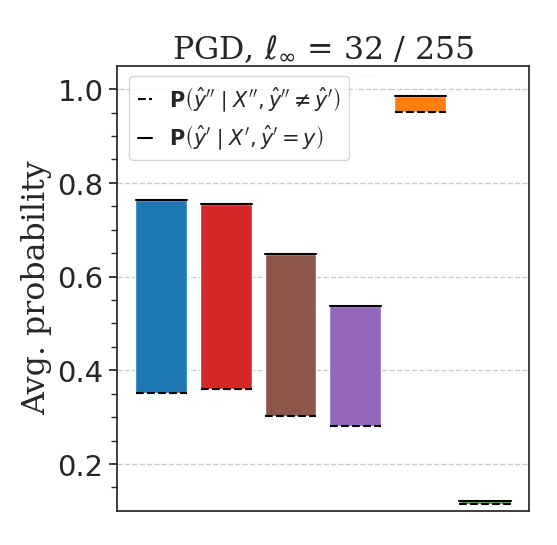
\includegraphics[width=\textwidth]{img/results_discussion/adversarial/DIFF_PGD_0.1255.png}
    \end{subfigure}
    \hfill
    \begin{subfigure}[b]{0.3\textwidth}
        \centering
        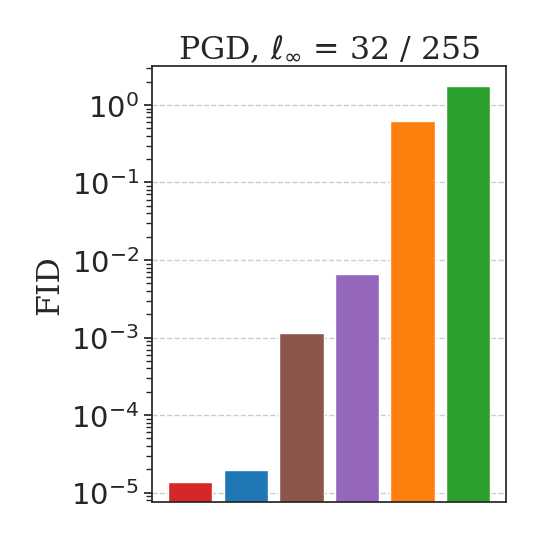
\includegraphics[width=\textwidth]{img/results_discussion/adversarial/FID_barplot_0.1255.png}
    \end{subfigure}
    \begin{subfigure}[b]{0.3\textwidth}
        \centering
        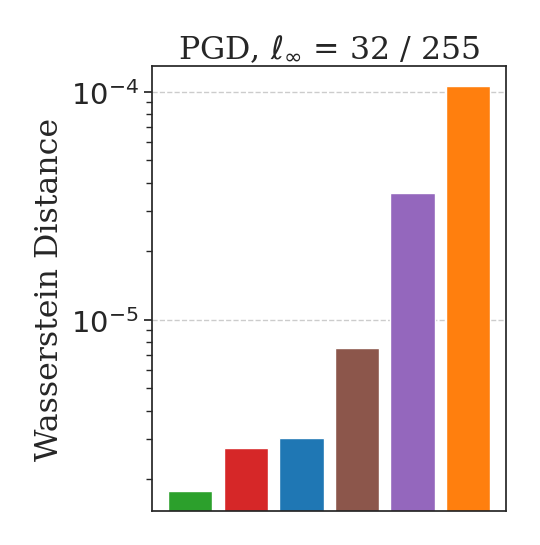
\includegraphics[width=\textwidth]{img/results_discussion/adversarial/W_barplot_0.1255.png}
    \end{subfigure}

    \vspace{1em}

    \begin{subfigure}[b]{0.3\textwidth}
        \centering
        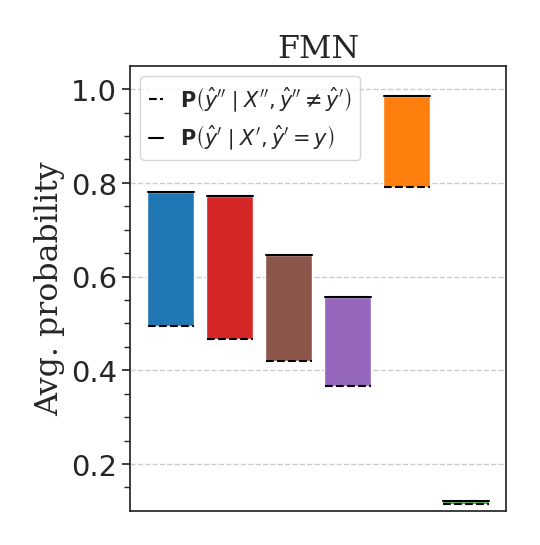
\includegraphics[width=\textwidth]{img/results_discussion/adversarial/DIFF_FMN.png}
    \end{subfigure}
    \hfill
    \begin{subfigure}[b]{0.3\textwidth}
        \centering
        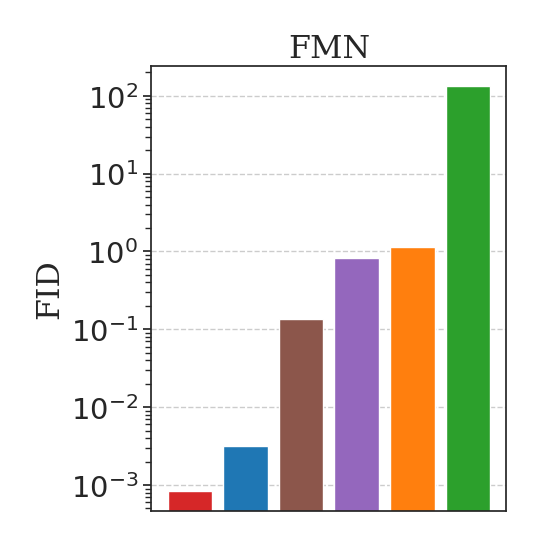
\includegraphics[width=\textwidth]{img/results_discussion/adversarial/FID_barplot_FMN.png}
    \end{subfigure}
    \begin{subfigure}[b]{0.3\textwidth}
        \centering
        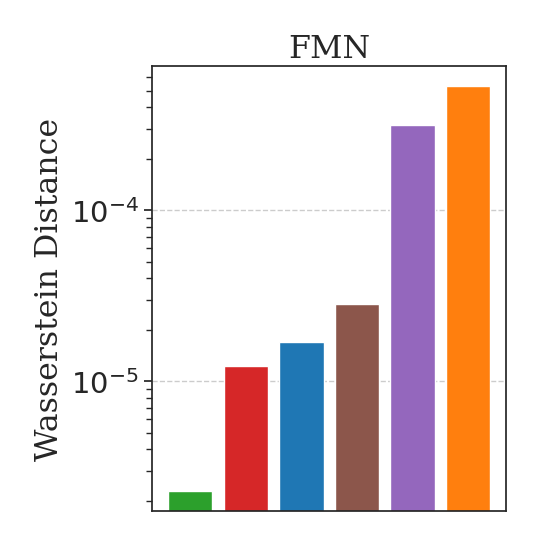
\includegraphics[width=\textwidth]{img/results_discussion/adversarial/W_barplot_FMN.png}
    \end{subfigure}

    \caption{
    The two metrics considered are FID, which amounts to the group-based dissimilarity 
    in the feature space, and Wasserstein distance, which measures the average distance between 
    probability distributions. 
    }
    \label{fig:adv_metric_comparison}
\end{figure}

Figure \ref{fig:adv_metric_comparison} displays some of these metrics for
PGD and FMN attacks, together with a condensed visualization of the average 
probability gap existing amidst predictions on original and adversarial examples. As
we can see, the discriminative power of these metrics stems from the overall difference 
between posteriors at $\beta = 1$. This result is not surprising, since the discriminant function 
of the classifier is constituted by a small subset of layers in the network, and is not expected 
to represent a complex discrimination that cannot be inferred from the distribution 
of samples in the feature space. As expected, probability-based metrics tend to concide in 
their assessment in general terms, and feature-space-based metrics as well. Besides, it is also not
surprising that feature space distances are more sensitive to the success rate of the attack, 
given that the inductive bias remains constant under any condition, whereas confidence-based metrics
are susceptible to the overall shift in the posterior, which in general favours non-informative
posteriors. A deeper insight into the evolution of these metrics for PGD and FMN attacks under increasing
adversarial ratio can be found in Figures \ref{fig:comparison_prob_metrics} and 
\ref{fig:comparison_feat_metrics}. \\

The results obtained in this section showcase the rationale behind the maximization of posterior
agreement, which can be thought of a surrogate version of the maximization of the mutual information
between original and perturbed datasets
\cite{buhmannDataScienceAlgorithms2022}. From an information-theoretic perspective, 
the maximization of mutual information effectively
distillates the information contained in the posterior distributions to that 
which is relevant for robustness assessment. This property is the source of the 
discriminative power displayed by PA and constitutes a fundamental difference
with respect to the baseline accuracy-based metrics considered.


\section{Out-of-distribution setting}\label{results_domain_generalization}

Following the analysis conducted in the previous section, the discriminability of PA
will be now explored in the domain generalization setting, which is a priori more convenient
for PA for being accuracy-based metrics less informative in this context. This is because
we are ultimately assessing the quality of the inductive bias of the model
by its ability to generalize to target (i.e. unseen) domains. In this sense, the additional
insight and discriminability exhibited by PA is expected to be more relevant for the selection of
models that perform well not only on unseen data, but also on unseen data that shares limited 
features with the training data. Under these conditions, the overlap between posteriors is more
informative than simply matching predictions (e.g. $\operatorname{AFR}_{\text{P}}$), because 
significant disagreement in
the remaining classes indicates vulnerability to distribution shifts present in
the source domains, which implies vulnerability to target domains as well. This is
a fundamental difference with respect to the adversarial setting, in which the nature of the
perturbation made posteriors less relevant for the robustness assessment.\\

This section will not address epoch-wise model selection, but will focus instead on 
the evaluation of the generalization capabilities of different learning algorithms under increasing 
levels of distribution shift, by computing the posterior agreement between source environments for 
models achieving maximum validation accuracy. More specifically, a baseline vanilla ERM algorithm will be 
used to train a ResNet18 model and will be compared with two robust 
learners, namely invariant risk minimization (IRM) and selective
augmentation (LISA), both introduced in Section \ref{sec:robust_learners}. Results should
ellucidate whether PA is able to discern datasets subjected to different levels of domain shift and
whether models achieving highest PA scores perform better on new domains. \\

Experiments will be performed by means of the DiagViB-6 dataset
framework
\cite{euligDiagViB6DiagnosticBenchmark2021}, 
which comprises MNIST images of size 128x128 within an augmentation pipeline enabling
the modification of six specific image factors: shape, hue, lightness, position,
scale and texture. Several variations in the \texttt{diagvibsix}
library\footnote{https://github.com/viictorjimenezzz/diagvibsix/tree/librarization}
have been implemented with the purpose 
of this project so that datasets can be built with a specific configuration of factors for each sample, which 
allows for a wide range of experiments in the data shift assessment and model selection settings. In
an analogous way to the adversarial case, datasets will be incrementally perturbed by including only
a fraction of the shifted samples, which in this context we will call shift ratio (SR).\\

Following the notation introduced in Section \ref{sec:domain_generalization_setting}, Definition 
\ref{def:shifted_factors_experiment} provides a characterization of source and target domains and
the randomness entailed by each dataset. The control over these aspects is the rationale behind
this experimental setup, since it is through synthetic image manipulation that we can maximize
invariant feature learning possibilities during training while providing optimal robustness
assessment conditions in validation and testing. Since changes in image factors can be independently 
introduced to each sample, the shifted dataset contains the same samples and in the same order
as the original dataset, thus removing sampling randomness contributions from the robustness score. 
Table \ref{tab:data_shift_table} stipulates the specific factors conforming each environment in this
experiment and Figure \ref{fig:data_shift_images} illustrates them with some examples.

CITE MORE INFO IN \ref{def:diagvib6_experiments} \\

\begin{definition}[Shifted factors experiment]\label{def:shifted_factors_experiment}
    The classification task involves the prediction of the shape factor (i.e. the digit)
    of handwritten fours and nines from the MNIST dataset. In particular, source and target
    domains are generated as follows:

    $$
    \begin{aligned}
        &\mathcal{S} = \{ X_0, X_1\},\\
        &\mathcal{T} = \{ X_1, X_2, X_3, X_4, X_5\},
    \end{aligned}
    $$

    where $X_j$ represents the random variable associated to domain $j$, 
    being $j$ the number of shifted factors with respect to domain $X_0$. 
    Datasets are generated by considering
    four different realizations of the experiment, namely $\tau_0^{\text{train}}$, $\tau_1^{\text{train}}$, $\tau^{\text{val}}$
    and $\tau^{\text{test}}$, each sampling from disjoint subsets of MNIST. Following the notation introduced
    in Chapter \ref{sec:experimental_setup}, we can define:
    $$
    \begin{aligned}
        &D^{\text{train}} = \{\bm{x}_0^{\text{train}}, \bm{x}_1^{\text{train}}\}, \; \text{where } \bm{x}_j := \bm{x}_j \circ \tau_j^{\text{train}}, \;j = 0,1 \\
        &D^{\text{val}} = \{\bm{x}_0^{\text{val}}, \bm{x}_1^{\text{val}}\}, \; \text{where } \bm{x}_j := \bm{x}_j \circ \tau^{\text{val}}, \;j=0,1 \\
        &D_j^{\text{test}} = \{\bm{x}_j^{\text{test}}\}, \; \text{where } \bm{x}_j^{\text{test}} := \bm{x}_j^{\text{test}} \circ \tau^{\text{test}}, \;j = 1,\dots,5
    \end{aligned}
    $$

    In this way, only training data is subject to both sampling randomness ($\tau_0^{\text{train}} \neq \tau_1^{\text{train}}$)
    and domain shift ($X_0 \nsim X_1$), emulating the conditions of real-world sampling experiments.
    In contrast, validation and testing datasets entail each a single noise instantiation, 
    which means that distribution shift is the only accountable source of randomness.
    Overall, two sets of $40\,000$ images for training, two sets of $20\,000$ 
    images for validation, and six sets of $10\,000$ images for testing are generated. 
\end{definition}

\begin{table}[H]
    \centering
    \begin{tabular}{l|c|c|c|c|c|c}
    \# Shift Factors & 0 & 1 & 2 & 3 & 4 & 5 \\
    \midrule
    Hue & red & \textbf{blue} & blue & blue & blue & blue \\
    Lightness & dark & dark & \textbf{bright} & bright & bright & bright \\
    Position  & CC & CC & CC & \textbf{LC} & LC & LC \\
    Scale  & normal & normal & normal & normal & \textbf{large} & large \\
    Texture & blank & blank & blank & blank & blank & \textbf{tiles} \\
    \textit{Shape} & \textit{4,9} &  \textit{4,9} &  \textit{4,9} & \textit{4,9} & \textit{4,9} & \textit{4,9} \\
    \bottomrule
    \end{tabular}
    \caption{
    Image factors associated to each of the environments considered in this experiment. CC and LC account
    for 'centered center' and 'centered low', respectively.
    }
    \label{tab:data_shift_table}
\end{table}


\begin{figure}[H]
    \centering
    \begin{subfigure}[b]{0.2\textwidth}
        \centering
        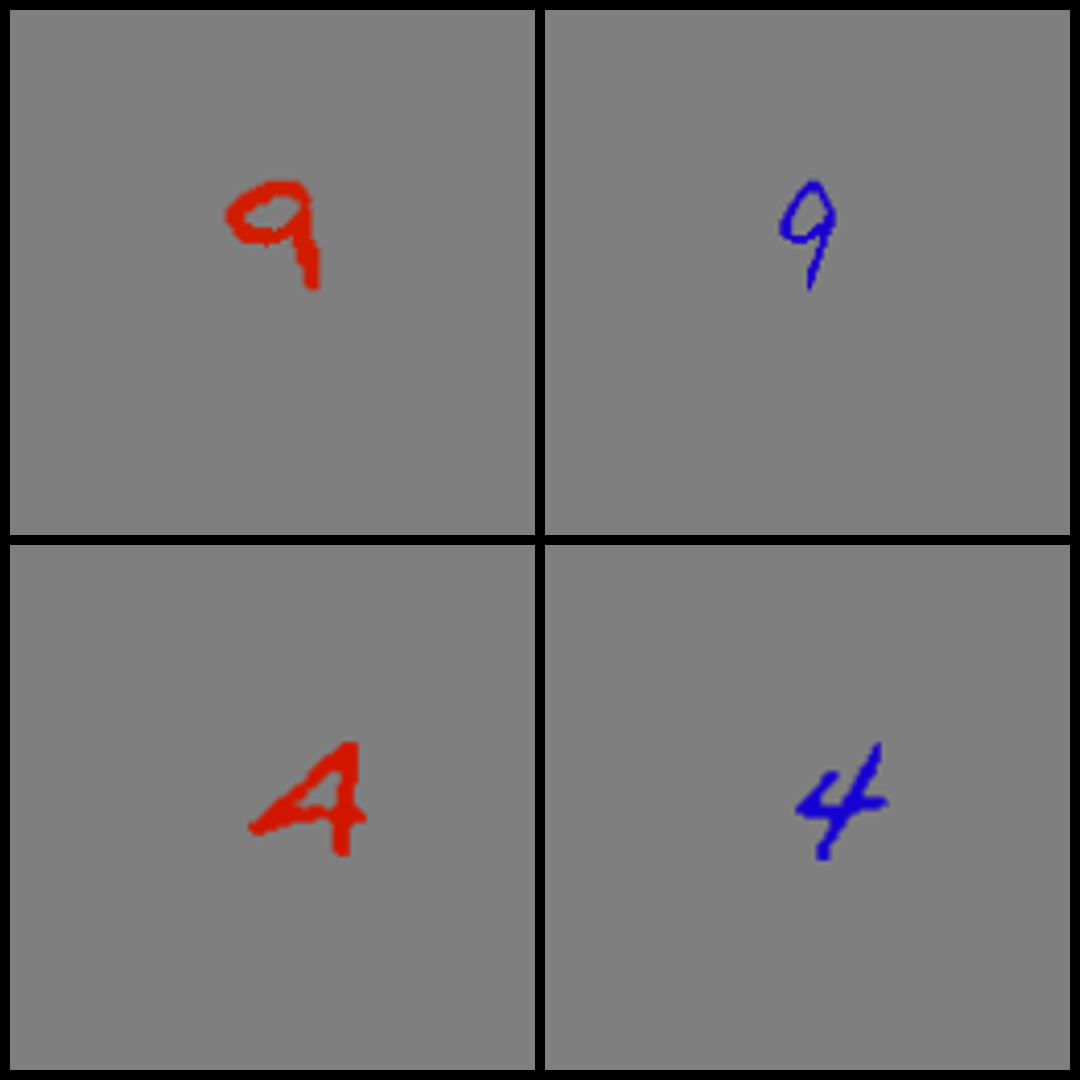
\includegraphics[height=2cm]{img/results_discussion/datashift/dsimages/train_collage.png}
        \caption*{Train}
    \end{subfigure}%
    \hfill
    \begin{subfigure}[b]{0.2\textwidth}
        \centering
        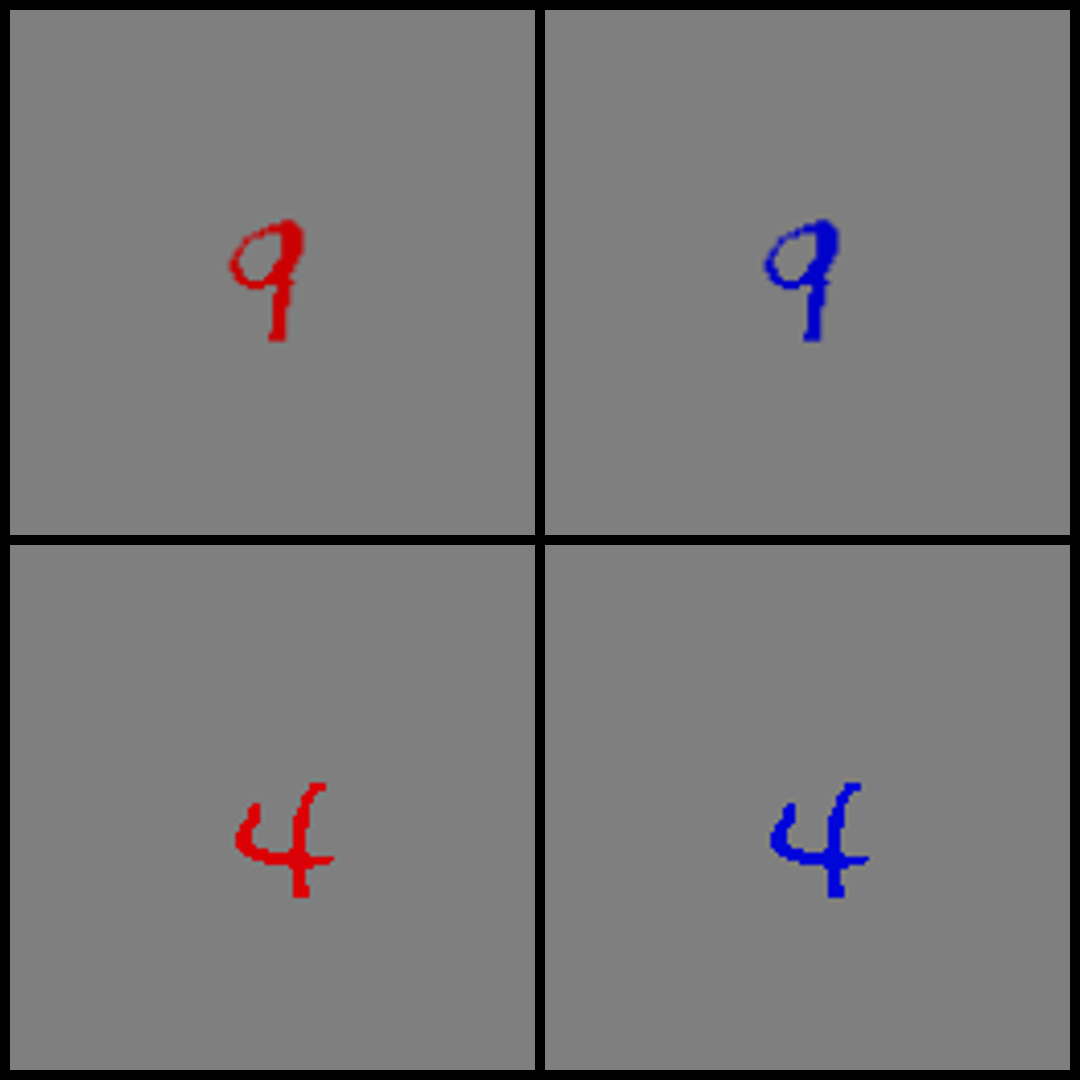
\includegraphics[height=2cm]{img/results_discussion/datashift/dsimages/val_collage.png}
        \caption*{Validation}
    \end{subfigure}%
    \hfill
    \begin{subfigure}[b]{0.6\textwidth}
        \centering
        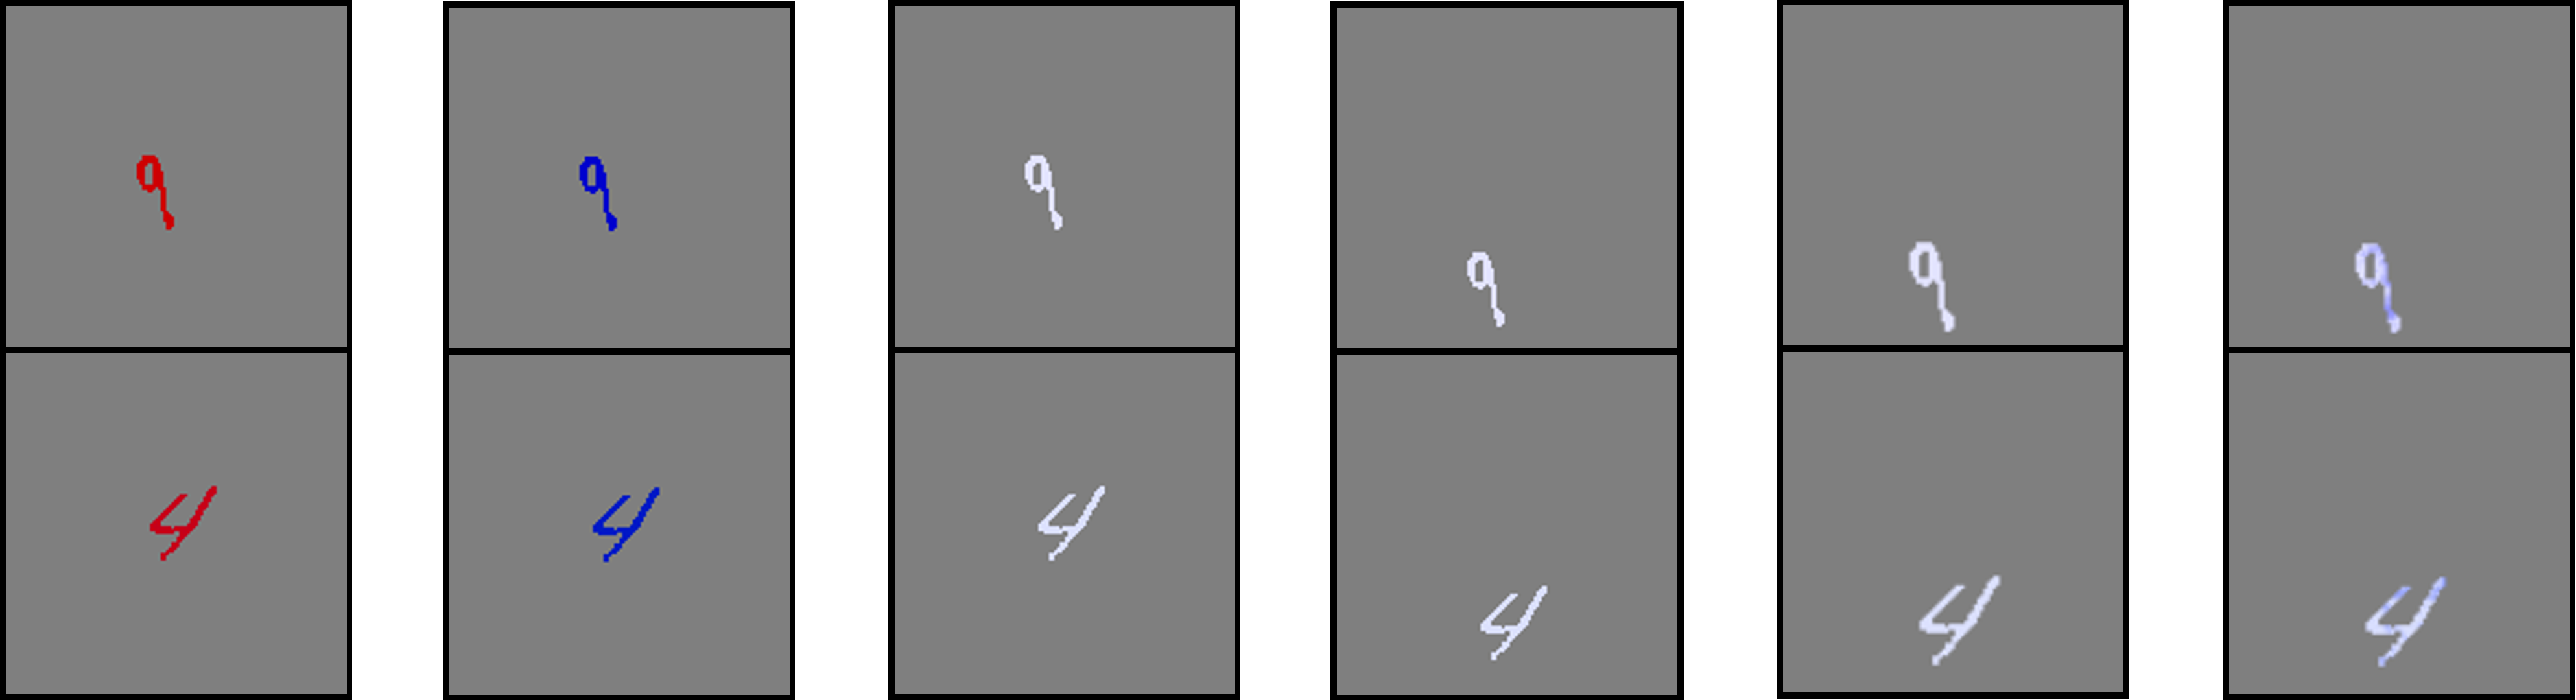
\includegraphics[height=2cm]{img/results_discussion/datashift/dsimages/test_collage2.png}
        \caption*{Test (1 - 5)}
    \end{subfigure}
    \caption{
    Illustration of the training, validation and test datasets. Samples for each
    training environment belong to different MNIST subsets, whereas samples of
    validation and test are corresponding.
    }
    \label{fig:data_shift_images}
\end{figure}


Results obtained in this setup show that PA succeeds at discriminating the 
different models by their predictive response under increasing number of shifted samples and 
under increasing shift power. In particular, ERM can be identified to be non-robust by the fact 
that its score is maximum for the first shifted factor, but decays rapidly to the minimum value 
after the second factor. In contrast, IRM and LISA show a reduced rate of decay and even display a
slight increase in performance for the last shift factor. \\

\begin{figure}[H]
    \centering
    \begin{subfigure}[b]{0.3\textwidth}
        \centering
        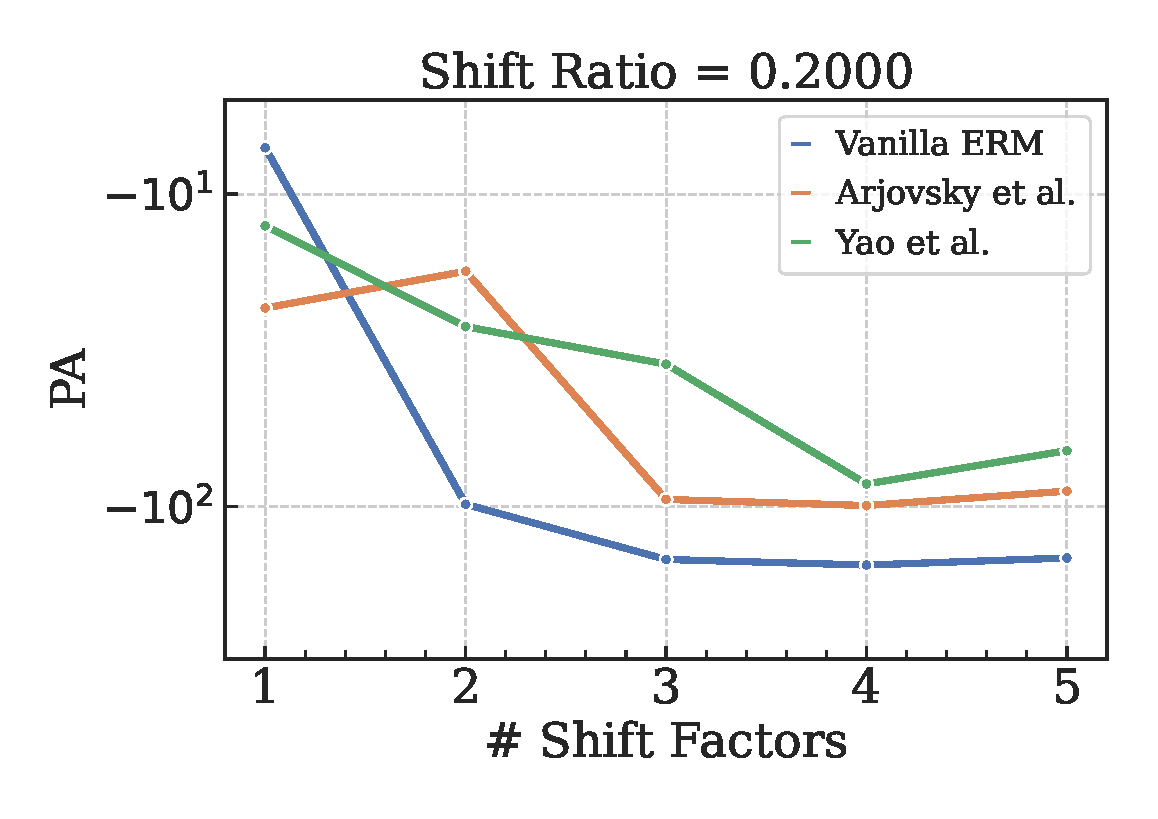
\includegraphics[width=\textwidth]{img/results_discussion/datashift/shift_ratio=0.200.pdf}
    \end{subfigure}
    \hfill
    \begin{subfigure}[b]{0.3\textwidth}
        \centering
        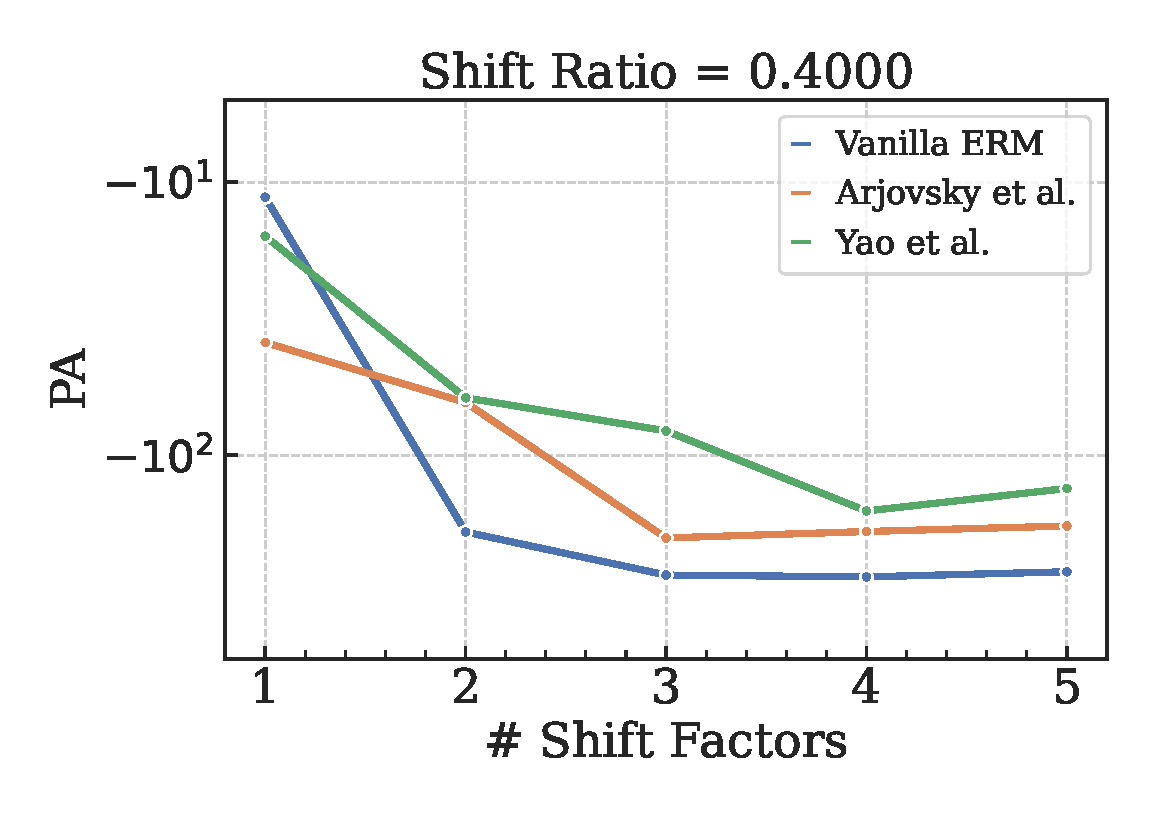
\includegraphics[width=\textwidth]{img/results_discussion/datashift/shift_ratio=0.400.pdf}
    \end{subfigure}
    \hfill
    \begin{subfigure}[b]{0.3\textwidth}
        \centering
        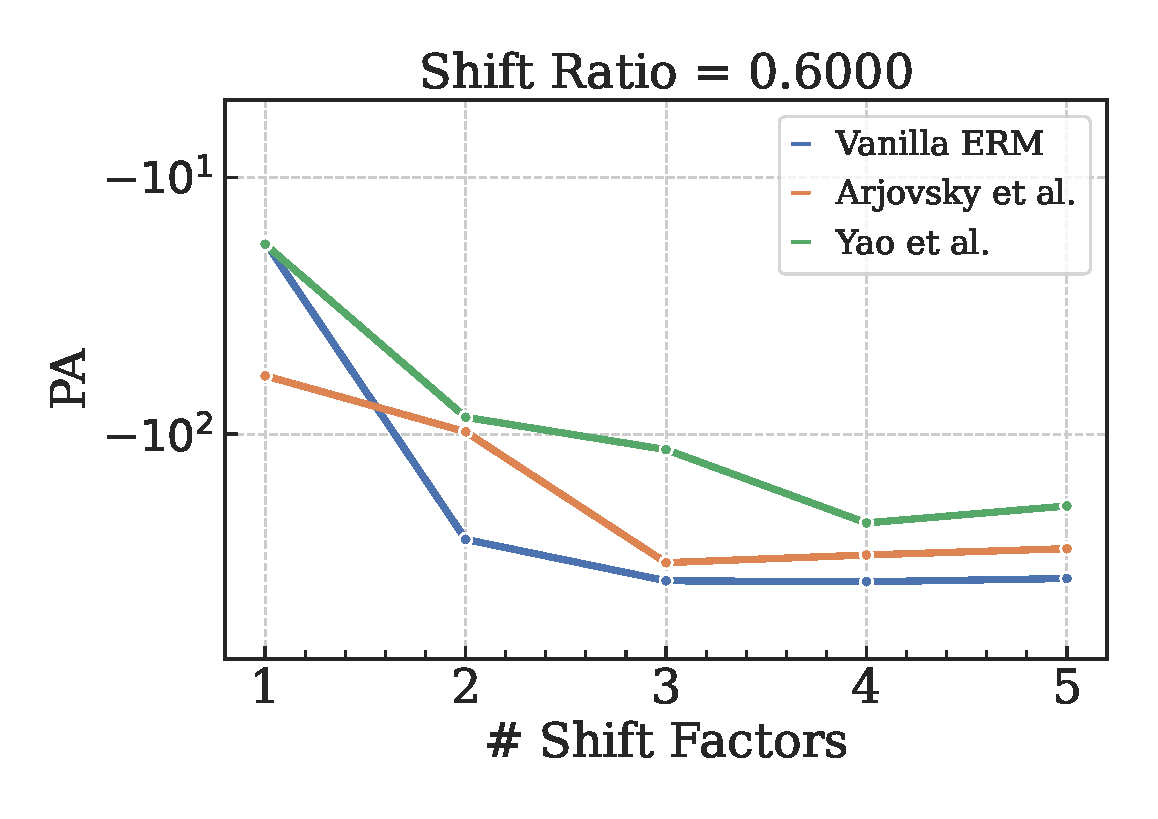
\includegraphics[width=\textwidth]{img/results_discussion/datashift/shift_ratio=0.600.pdf}
    \end{subfigure}

    \vspace{1em}

    \begin{subfigure}[b]{0.3\textwidth}
        \centering
        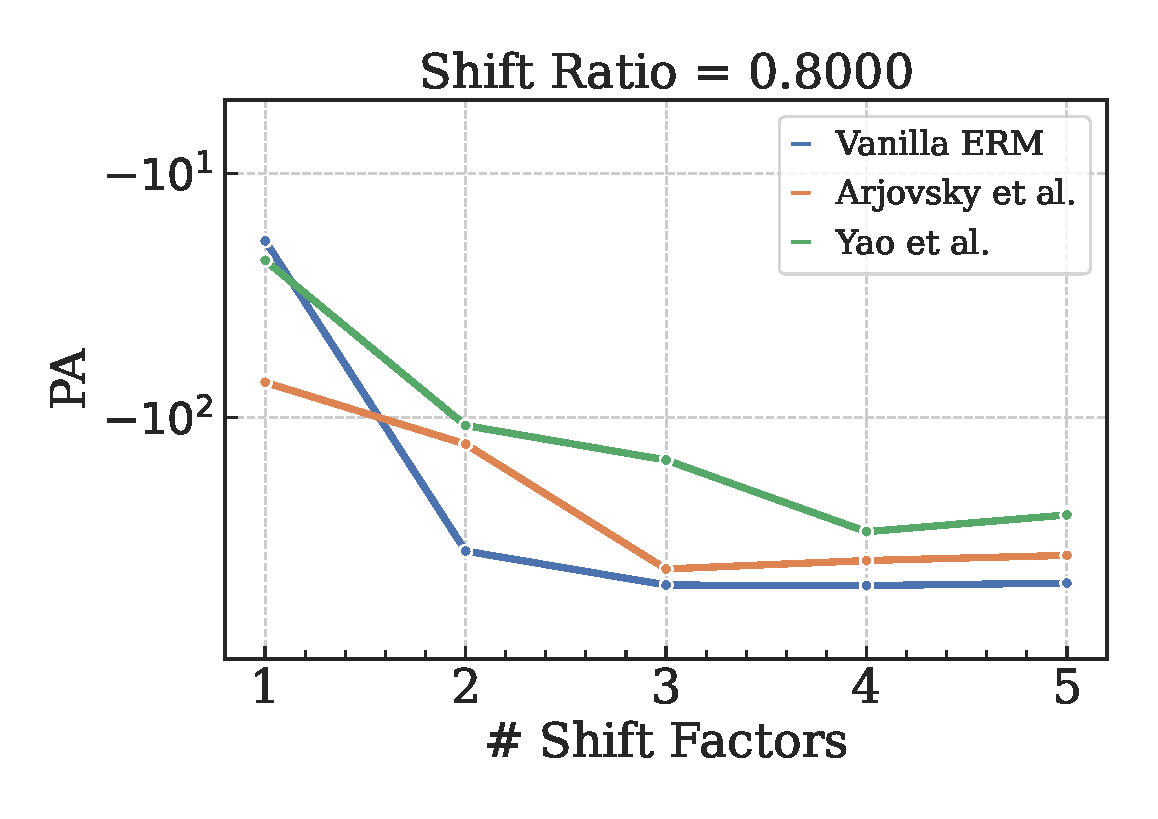
\includegraphics[width=\textwidth]{img/results_discussion/datashift/shift_ratio=0.800.pdf}
    \end{subfigure}
    \hspace{13pt}
    \begin{subfigure}[b]{0.3\textwidth}
        \centering
        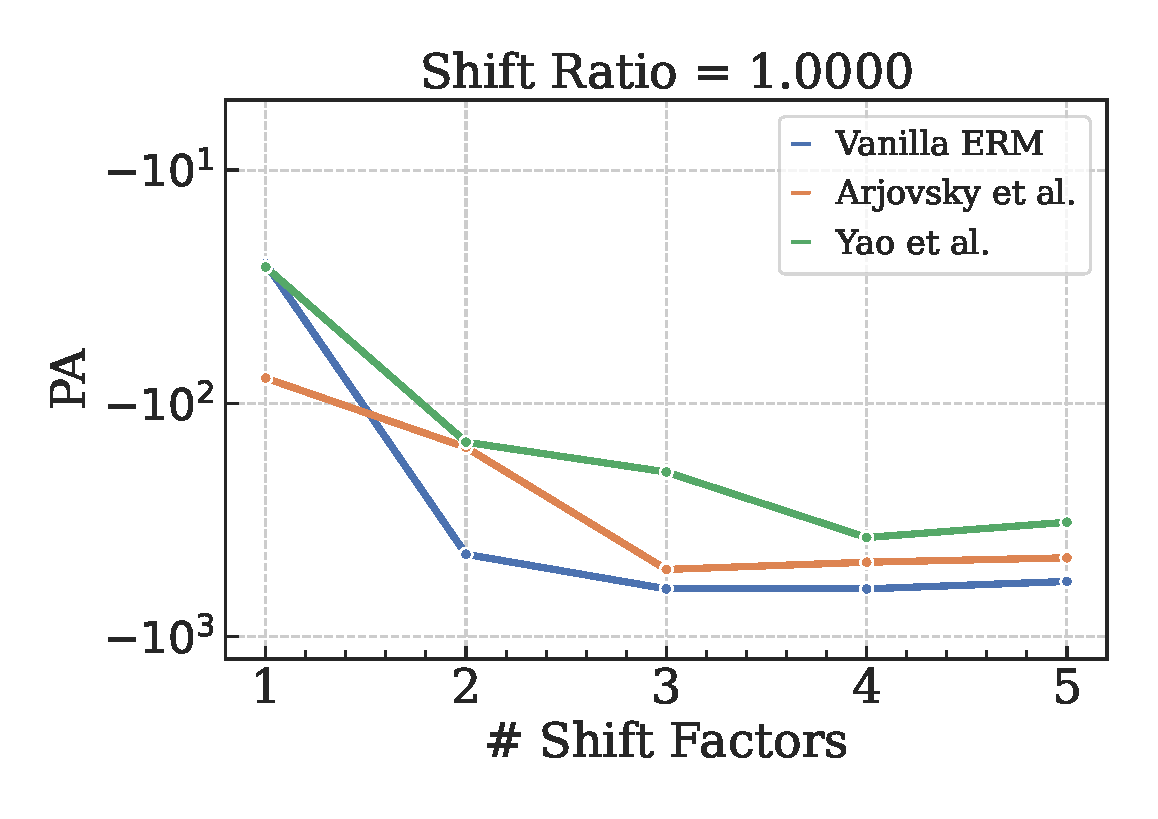
\includegraphics[width=\textwidth]{img/results_discussion/datashift/shift_ratio=1.000.pdf}
    \end{subfigure}

    \caption{Evolution of PA under increasing levels of shift power. Weights maximizing validation
    accuracy were selected for ERM, IRM and LISA algorithms. Results for incremental presence of shifted
    samples indicate that PA is able to differentiate weak and robust models.
    }
    \label{fig:six_figures}
\end{figure}

The unexpected increase in PA after four shifted factors seems
inconsistent with the alleged non-increasing behaviour of PA, as per
Section \ref{sec:robustness_to_covariate_shift}. Nevertheless, this phenomenon 
only highlights that robustness does not stem from the data generation process but instead 
from the latent representation of the model and the features selected for the construction 
of its inductive bias, as discussed in the introductive chapter. In this particular case, 
Table \ref{tab:CS_shift} shows that
there is a clear discontinuity in the feature representation of the data when the texture
factor is shifted, which results in a different discriminator function that ultimately
leads to a predictive behaviour that aligns slightly better with the original predictions. \\

\begin{table}[H]
    \centering
    \begin{tabular}{l|c|c|c|c|c}
    \# Shift Factors & 1 & 2 & 3 & 4 & 5 \\
    \midrule
    {\color{tab:blue} \textbf{Vanilla ERM}} & 0.9978 & 0.9303 & 0.9562 & 0.9561 & \textbf{0.6661} \\
    {\color{tab:orange} \textbf{Arjovsky et al.}} & 0.9967 & 0.9018 & 0.9296 & 0.9374 & \textbf{0.5585} \\
    {\color{tab:green} \textbf{Yao et al.}}  & 0.9980 & 0.9431 & 0.9431 & 0.9641 & \textbf{0.7130} \\
    \bottomrule
    \end{tabular}
    \caption{
    Pairwise cosine similarity between feature space representations of original and
    augmented images, for each of the shifted datasets. The abrupt decrease in similarity
    for the fifth environment indicates a discontinuity in the feature representation of images,
    which leads to non-comparable predictive outcomes.
    }
    \label{tab:CS_shift}
    \end{table}


% - Here explain that PA can also be approximated by considering $\beta$ a fixed beta and evaluating
% in many environments. This validity of this approximation will be higher the lower is the decrease
% in performance of the model under increasing shift power. In any case, the assessment won't be optimal
% but can be used to spare computational ressources. Figure \ref{fig:datashift_eval_pa} shows the evaluated PA (i.e. $\beta^{*}$ computed only for the
% first two environments) for each model against the standard accuracy displayed during the whole
% optimization process. \\


% \begin{figure}[H]
%     \centering
%     \begin{subfigure}[b]{0.45\textwidth}
%         \centering
%         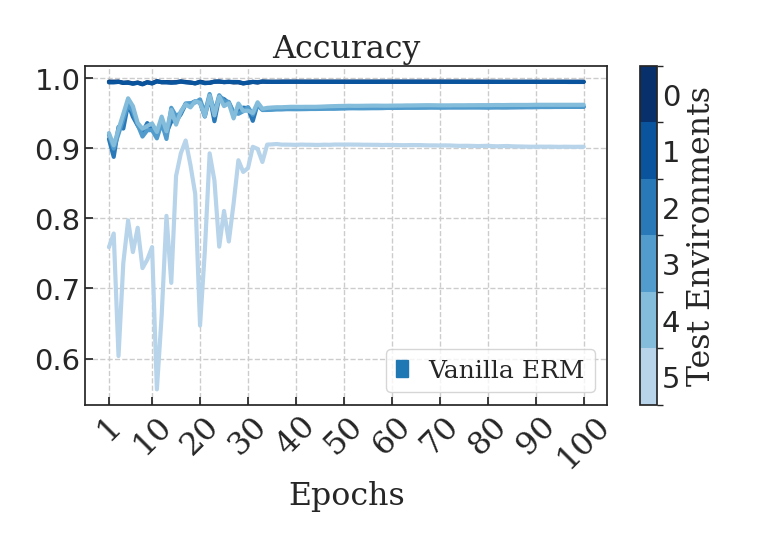
\includegraphics[width=\textwidth]{img/results_discussion/datashift/paper_oracle_all_erm.png}
%     \end{subfigure}
%     \hfill
%     \begin{subfigure}[b]{0.45\textwidth}
%         \centering
%         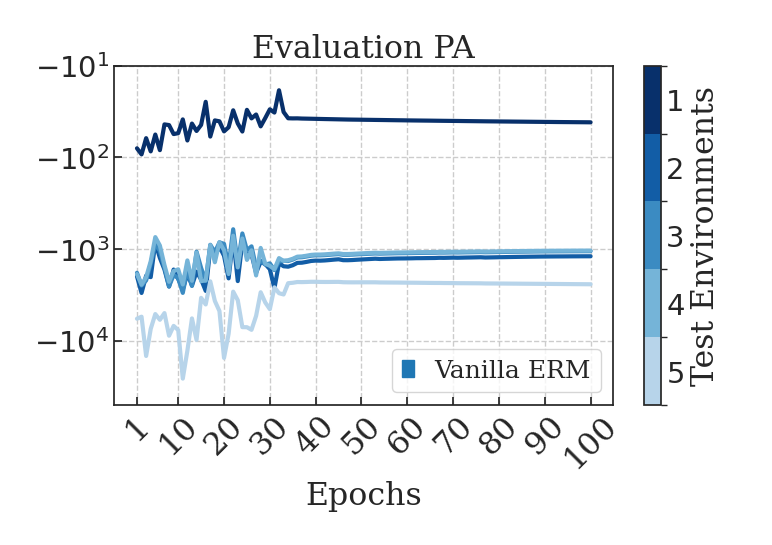
\includegraphics[width=\textwidth]{img/results_discussion/datashift/paper_PA_all_erm.png}
%     \end{subfigure}

%     \vspace{1em}

%     \begin{subfigure}[b]{0.45\textwidth}
%         \centering
%         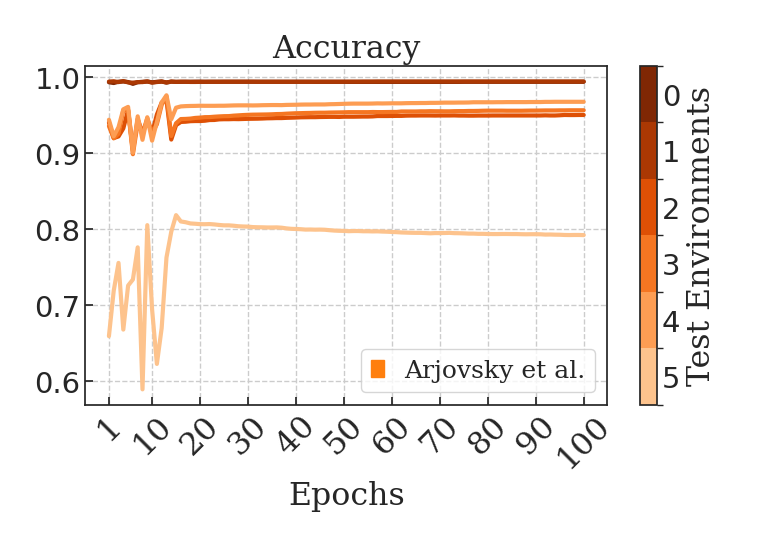
\includegraphics[width=\textwidth]{img/results_discussion/datashift/paper_oracle_all_irm.png}
%     \end{subfigure}
%     \hfill
%     \begin{subfigure}[b]{0.45\textwidth}
%         \centering
%         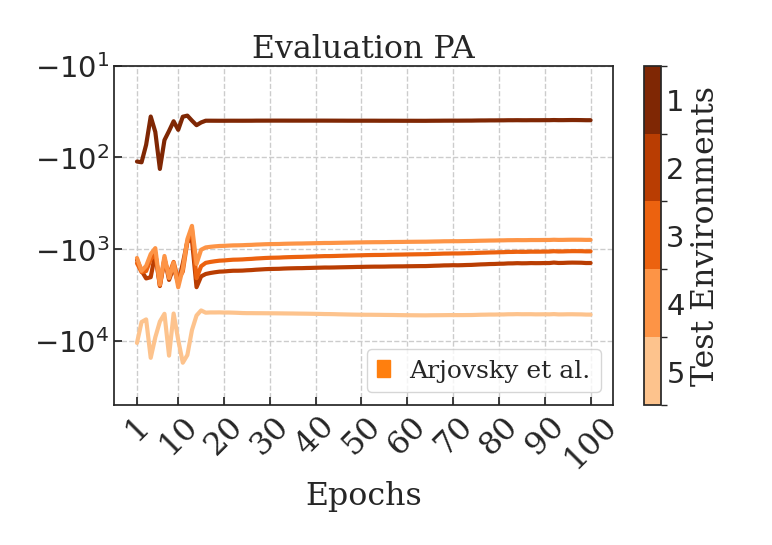
\includegraphics[width=\textwidth]{img/results_discussion/datashift/paper_PA_all_irm.png}
%     \end{subfigure}

%     \caption{PA evaluation.}
%     \label{fig:datashift_eval_pa}
% \end{figure}

% \begin{figure}
%     \centering
%     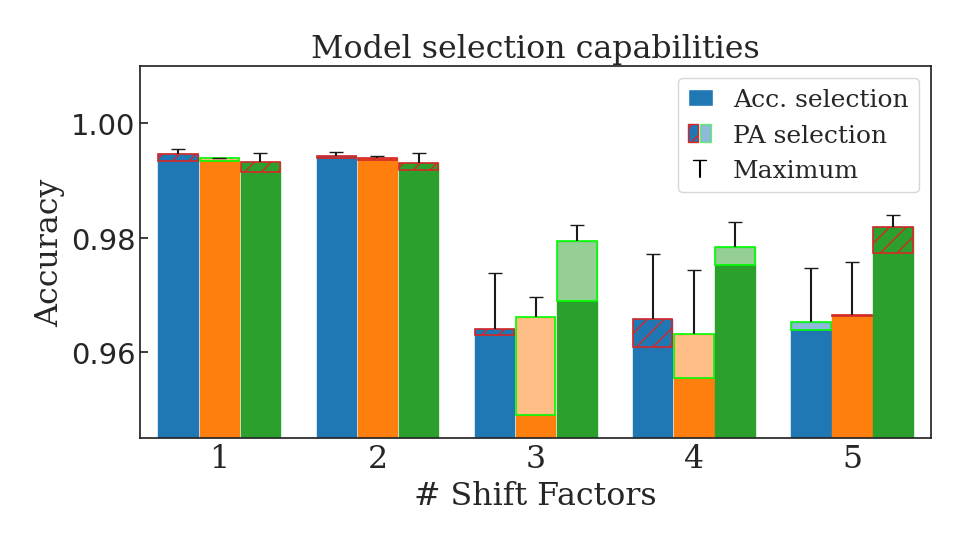
\includegraphics[width=0.7\textwidth]{img/results_discussion/datashift/model_selection.png}
%     \caption{Model selection capabilities.}
%     \label{fig:model_selection_capabilities}
% \end{figure}



\begin{table}[h]
    \centering
    \resizebox{\textwidth}{!}{%
    \begin{tabular}{l|ccc|ccc|ccc}
    \multirow{2}{*}{} & \multicolumn{3}{c|}{1 Shifted Factor} & \multicolumn{3}{c|}{3 Shifted Factors} & \multicolumn{3}{c}{5 Shifted Factors} \\
     & PA & $\operatorname{AFR}_{\text{P}}$ & $\operatorname{AFR}_{\text{T}}$ & PA & $\operatorname{AFR}_{\text{P}}$  & $\operatorname{AFR}_{\text{T}}$ & PA & $\operatorname{AFR}_{\text{P}}$  & $\operatorname{AFR}_{\text{T}}$ \\
    \midrule
    {\color{tab:blue} \textbf{Vanilla ERM}} & \textbf{-24.91}  & 0.999 & 0.993 & -625.6 & 0.979 & 0.975 & -579.38 & 0.976 & 0.873 \\
    {\color{tab:orange} \textbf{Arjovsky et al.}} & -76.76 & 0.998 & 0.993 & -514.2 & 0.976 & 0.978  & -464.2 & 0.976 & 0.911 \\
    {\color{tab:green} \textbf{Yao et al.}} & -26.21 & \textbf{0.999} & \textbf{0.994} & \textbf{-201.2} & \textbf{0.985} & \textbf{0.980} & \textbf{-324.4} & \textbf{0.988} & \textbf{0.945} \\
    \bottomrule
    \end{tabular}
    }
    \caption{
        Comparison of PA, $\operatorname{AFR}_{\text{P}}$ and $\operatorname{AFR}_{\text{T}}$ scores
        for ERM, IRM and LISA learning algorithms under different levels of shift power. The highest robustness 
        score is emboldened for every case. PA is able to discriminate algorithms consistently and distinguish
        the first shifted factor, which is seen by the model during training, from the rest.
    }
    \label{tab:shift_comparison_table}
\end{table}

% As shown in Figure \ref{fig:datashift_selection}, PA-based model selection behaves differently in robust
% and non-robust algorithms. Following the reasoning derived in previous sections, it is likely that the PA
% assessment on ERM is mostly driven by standard generalization error, due to the fact that ERM is agnostic
% of the environment to which each sample belongs to and therefore to the accountable source of randomness represented
% by the environment shift. The risk minimization problem under these conditions should give rise to less informative
% predictive outcomes, given that the domain-invariant features associated with the task are less accessible, and
% thus reduce the penalization weight of mismatching samples. This intuition is supported by the fact that ERM
% optimization yields models that performs worse in all test datasets than the ones obtained through IRM,
% as can be seen in Figure \ref{fig:datashift_eval_pa}. Besides, results show that the selected model for ERM 
% performs better an all metrics for the first test environment, which contains
% the same factor configuration as one of the validation environments, and maintains or slightly decreases its performance
% for increasing levels of shift. In addition, the PA-selected model appears to encode a slight variation of the 
% decision rule from that of the accuracy-selected model, given that samples near to the decision boundary are now
% more likely classified as nines than fours, which increases specificity as much as it decreases sensitivity. \\

% Regarding PA-based model selection in robust learners, we observe the opposite behaviour. Since models are more likely
% to represent domain-invariant features, each with its distinctive strategy, predictive outcomes are expected to
% be more informative and thus increase the penalization contribution of mismatching samples, which will be the ones
% containing domain-invariant features that are not sufficiently considered in the inductive bias of the model. PA
% model selection under these conditions is thus more likely to favor sets of weights that perform better under
% increasing levels of shift, at the expense of losing predictive power on the environments in which it operated. 
% Results align with this interpretation, as we observe a notable increase in performance across all shifted datasets
% with respect to the accuracy-selected model, especially in the LISA case, at the expense of significantly decreasing
% performance on the first environment.\\


% \begin{figure}[H]
%     \centering
%     \begin{subfigure}[b]{0.6\textwidth}
%         \centering
%         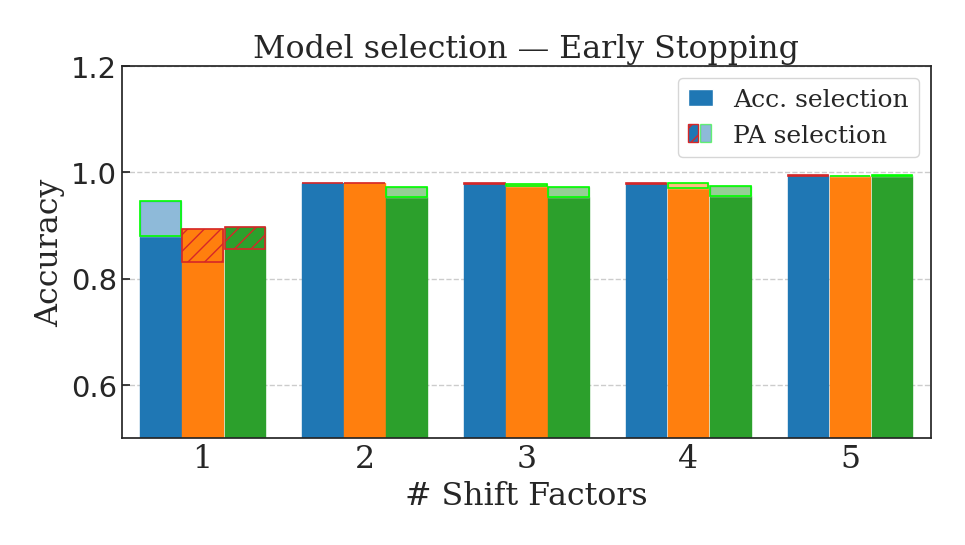
\includegraphics[width=\textwidth]{img/results_discussion/datashift/paper_selection_ppred=1.0_met=acc.png}
%     \end{subfigure}

%     \begin{subfigure}[b]{0.6\textwidth}
%         \centering
%         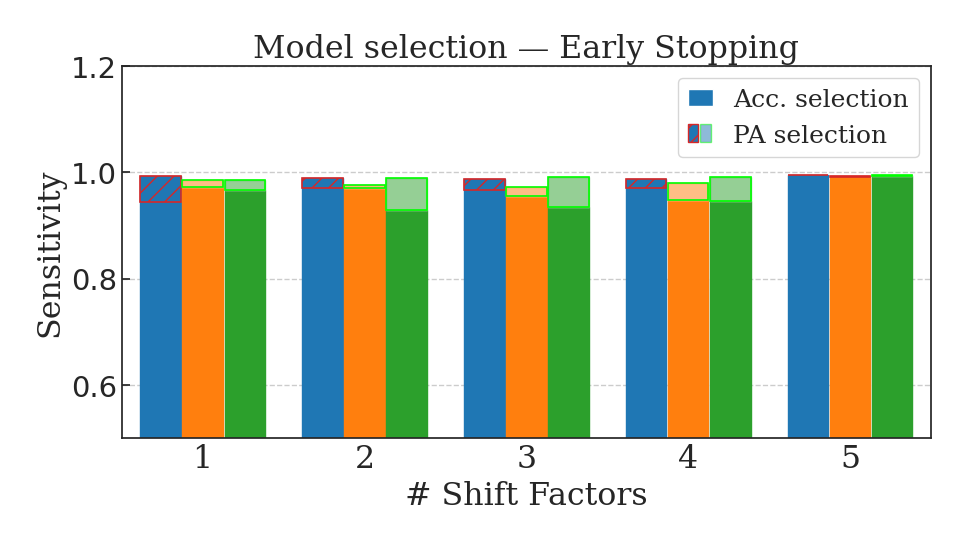
\includegraphics[width=\textwidth]{img/results_discussion/datashift/paper_selection_ppred=1.0_met=sensitivity.png}
%     \end{subfigure}

%     \begin{subfigure}[b]{0.6\textwidth}
%         \centering
%         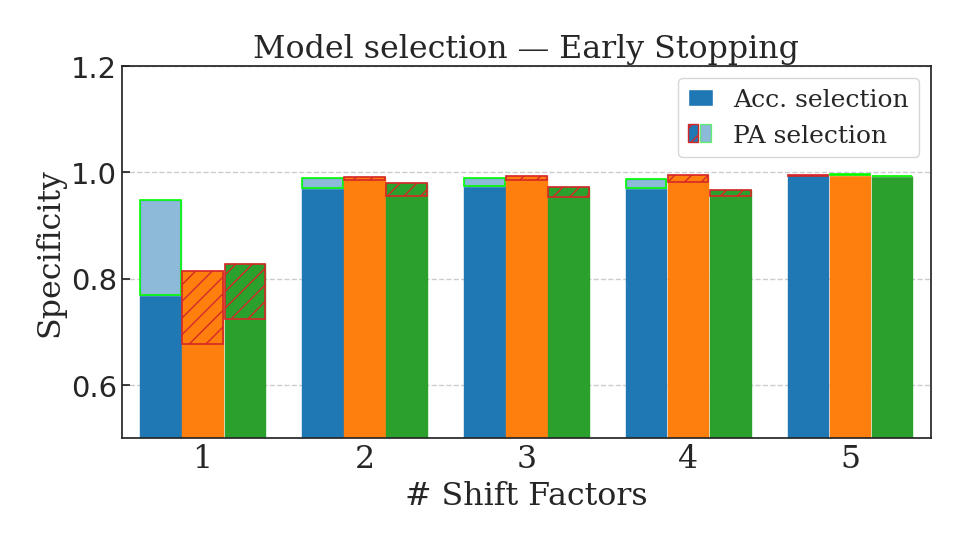
\includegraphics[width=\textwidth]{img/results_discussion/datashift/paper_selection_ppred=1.0_met=specificity.png}
%     \end{subfigure}
%     \caption{
%     Accuracy, sensitivity and precision displayed by sets of ResNet18 weights on
%     shifted test datasets, obtained through ERM, IRM and LISA
%     training procedures. Accuracy-based selection is compared to PA-based selection, both
%     operating with a validation dataset composed of samples of environments 0 and 1.
%     }
%     \label{fig:datashift_selection}
% \end{figure}



% Model:  0
% Accuracy:  [88.08000088 97.94499874 98.05499911 97.94499874 99.44000244]
% PA_diff:  [ 6.52999878e+00 -5.00082970e-03 -3.19999456e-01 -1.19996071e-01
%  -7.50005245e-02]
% Model:  1
% Accuracy:  [89.34500217 98.00500274 97.43499756 97.11999893 99.36000109]
% PA_diff:  [-6.13500476  0.          0.41000247  0.88000298  0.01499653]
% Model:  2
% Accuracy:  [89.74499702 95.35499811 95.3700006  95.59500217 99.32000041]
% PA_diff:  [-4.24499512  1.85500383  1.87000036  1.78999901  0.06999969]



% \begin{table}[H]
%     \centering
%     \resizebox{\textwidth}{!}{%
%     \begin{tabular}{l|cl|cl|cl|cl|cl|cl}
%     \multirow{2}{*}{} & \multicolumn{2}{c|}{\textbf{0}} & \multicolumn{2}{c|}{\textbf{1}} & \multicolumn{2}{c|}{\textbf{2}} & \multicolumn{2}{c|}{\textbf{3}} & \multicolumn{2}{c|}{\textbf{4}} & \multicolumn{2}{c}{\textbf{5}} \\
%     \textbf{{\color{tab:blue} \textbf{ERM}}} & Acc. & $\Delta_{\operatorname{PA}}$ & Acc. & $\Delta_{\operatorname{PA}}$ & Acc. & $\Delta_{\operatorname{PA}}$ & Acc. & $\Delta_{\operatorname{PA}}$ & Acc. & $\Delta_{\operatorname{PA}}$ & Acc. & $\Delta_{\operatorname{PA}}$ \\
%     \midrule
%     Specificity & 99.4 & \PlusMinus 0.01 & 68.0 & {\color{tab:green}  \textbf{\Plus 10.1}} & 45.2 & {\color{tab:red} \textbf{\Minus 10.1}} & 42.1 & {\color{tab:red} \textbf{\Minus 6.0}} & 42.9 & {\color{tab:red} \textbf{\Minus 9.3}} & 32.0 & {\color{tab:red} \textbf{\Minus 3.8}} \\
%     Sensitivity & \textbf{99.4} & \PlusMinus 0.01 & 67.1 & {\color{tab:red} \textbf{\Minus 7.9}} & 44.9 & {\color{tab:green}  \textbf{\Plus 0.8}} & 42.7 & {\color{tab:green}  \textbf{\Plus 1.3}} & 39.1 & {\color{tab:green}  \textbf{\Plus 1.5}} & 30.3 & {\color{tab:green}  \textbf{\Plus 1.4}} \\
%     \midrule
%     Accuracy & 88.1 & \PlusMinus 0.01 & 97.9 & \PlusMinus 0.01 & 98.1 & \PlusMinus 0.01 & 97.9 & \PlusMinus 0.01 & 42.5 & \PlusMinus 0.01 & 32.8 & \PlusMinus 0.01 \\
%     \midrule
%     \addlinespace
%     \addlinespace
%     \textbf{{\color{tab:orange} \textbf{IRM}}} & Acc. & $\Delta_{\operatorname{PA}}$ & Acc. & $\Delta_{\operatorname{PA}}$ & Acc. & $\Delta_{\operatorname{PA}}$ & Acc. & $\Delta_{\operatorname{PA}}$ & Acc. & $\Delta_{\operatorname{PA}}$ & Acc. & $\Delta_{\operatorname{PA}}$ \\
%     \midrule
%     Specificity & 99.4 & \PlusMinus 0.01 & 68.0 & {\color{tab:green}  \textbf{\Plus 10.1}} & 45.2 & {\color{tab:red} \textbf{\Minus 10.1}} & 42.1 & {\color{tab:red} \textbf{\Minus 6.0}} & 42.9 & {\color{tab:red} \textbf{\Minus 9.3}} & 32.0 & {\color{tab:red} \textbf{\Minus 3.8}} \\
%     Sensitivity & \textbf{99.4} & \PlusMinus 0.01 & 67.1 & {\color{tab:red} \textbf{\Minus 7.9}} & 44.9 & {\color{tab:green}  \textbf{\Plus 0.8}} & 42.7 & {\color{tab:green}  \textbf{\Plus 1.3}} & 39.1 & {\color{tab:green}  \textbf{\Plus 1.5}} & 30.3 & {\color{tab:green}  \textbf{\Plus 1.4}} \\
%     \midrule
%     Accuracy & 99.4 & \PlusMinus 0.01 & 59.3 & \PlusMinus 0.01 & 46.7 & \PlusMinus 0.01 & 44.9 & \PlusMinus 0.01 & 42.5 & \PlusMinus 0.01 & 32.8 & \PlusMinus 0.01 \\
%     \midrule
%     \addlinespace
%     \addlinespace
%     \textbf{{\color{tab:green} \textbf{LISA}}} & Acc. & $\Delta_{\operatorname{PA}}$ & Acc. & $\Delta_{\operatorname{PA}}$ & Acc. & $\Delta_{\operatorname{PA}}$ & Acc. & $\Delta_{\operatorname{PA}}$ & Acc. & $\Delta_{\operatorname{PA}}$ & Acc. & $\Delta_{\operatorname{PA}}$ \\
%     \midrule
%     Specificity & 99.4 & \PlusMinus 0.01 & 68.0 & {\color{tab:green}  \textbf{\Plus 10.1}} & 45.2 & {\color{tab:red} \textbf{\Minus 10.1}} & 42.1 & {\color{tab:red} \textbf{\Minus 6.0}} & 42.9 & {\color{tab:red} \textbf{\Minus 9.3}} & 32.0 & {\color{tab:red} \textbf{\Minus 3.8}} \\
%     Sensitivity & \textbf{99.4} & \PlusMinus 0.01 & 67.1 & {\color{tab:red} \textbf{\Minus 7.9}} & 44.9 & {\color{tab:green}  \textbf{\Plus 0.8}} & 42.7 & {\color{tab:green}  \textbf{\Plus 1.3}} & 39.1 & {\color{tab:green}  \textbf{\Plus 1.5}} & 30.3 & {\color{tab:green}  \textbf{\Plus 1.4}} \\
%     \midrule
%     Accuracy & 99.4 & \PlusMinus 0.01 & 59.3 & \PlusMinus 0.01 & 46.7 & \PlusMinus 0.01 & 44.9 & \PlusMinus 0.01 & 42.5 & \PlusMinus 0.01 & 32.8 & \PlusMinus 0.01 \\
%     \bottomrule
%     \end{tabular}%
%     }
%     \caption{REMOVEopt=adam-lr=0.0001-mf=hue-npair=FalseREMOVE Test performance on increasingly shifted datasets for models selected during ERM and IRM procedures. Different validation datasets are used, and the selection capabilities of PA and validation accuracy are compared.}
%     \label{tab:paper_msel}
%     \end{table}


\cleardoublepage
